%version of 12-11-19

\chapter{Graphs II:
Graphs for Computing and Communicating}
\label{ch:Graphs2}
\index{graph}

\begin{quote}
{\em Many hands make light work} \\ 
\hspace*{1in}John Heywood, 15th century English writer
\end{quote}

\bigskip

Chapter~\ref{ch:Graphs1} has laid the groundwork for an intensive study of the many  ways in which graphs and graph-related concepts find application within the fields of computing and communicating.  That chapter focused mainly on properties of graphs---and families of graphs---that are local and descriptive: What is the essence of a graph's being a tree? a hypercube?  The current chapter takes a further step and studies how the described local structure influences some of the dynamically applicable characteristics of graphs.  Two major foci in this chapter are {\em vertex-coloring} (Section~\ref{sec:graph-color}) and {\em path discovery} (Section~\ref{sec:path-cycle-problems}).  Both of these topics are used algorithmically in myriad applications of graphs, from circuit layout to computation scheduling to inter-agent communication scheduling.  We provide a layered presentation to both topics: We completely cover the basic aspects of both topics; we offer extended material in appendices, providing further study opportunities for the interested reader; and we provide pointers to the literature for a number of fascinating more-advanced topics.  We close the chapter with capsule discussions of several specialized topics which go beyond the scope of any introductory text.  We hope that the reader will be excited by these preliminary excursions into some of the wats that graph theory plays a role in ``real life".


%%%%%%%%%%%%%%%%%%%%%%%%%%%%%

\section{Graph Coloring and Chromatic number}
\label{sec:graph-color}
\index{graph!vertex-coloring}

\index{graph!chromatic number}

%This section introduces the notion of {\it graph coloring}, and its associated notion of the {\it chromatic number} of a graph.

\index{graph!vertex-coloring}
\index{graph!chromatic number}
 
A {\it vertex-coloring} of a graph $\g$ is an assignment of labels (the ``{\em colors}") to $\g$'s vertices,  in such a way that all of a vertex $v$'s neighbors get different labels than $v$'s.  The {\it chromatic number} of a graph $\g$ is the smallest number of colors that one can use in crafting a legal vertex-coloring of $\g$.  In traditional parlance, the assertions

\smallskip

``$\g$ has chromatic number $c$'' \ \ \ and \ \ \  ``$\g$ is {\it $c$-colorable}''

\index{graph!$c$-colorable}

\smallskip

\noindent
are viewed as synonymous.

\ignore{********
{\Denis I added the following remark, do you agree?}
This notion is an important characteristic of a graph.
It is like an intermediate concept between the degree (local)
and diameter (global), which are both easy to compute. 
Determining the chromatic number is not easy to compute for any graphs.
*********}

\bigskip

\noindent \fbox{ \begin{minipage}{0.96\textwidth}
The notion of graph coloring can be used to computational advantage in a broad variety of situations.

\medskip

One extremely important, and illustrative, use of graph coloring is to model independence among agents in {\it distributed} computing: The vertices of a computation-graph $\g$ represent {\it agents}, such as, e.g., processing elements in a multicomputer; and $g$'s edges represent {\it communication links} that enable each vertex $u$ to check its neighbors' states before taking any action and to inform its neighbors of state-changes occasioned by an action by $u$.  

\smallskip

The prohibition against ``monochrome'' edges---i.e., edges both of whose incident vertices have the same color---guarantees that vertex $u$ and all of its like-colored vertices can act at the same instant with no fear of missing an important input to those actions.  Indeed, one often encounters programs for distributed computing that look something like

\smallskip

1. All {\em red} vertices perform simultaneously an action

2. All {\em green} vertices perform simultaneously an action

3. All {\em blue} vertices perform simultaneously an action

$\cdots$

%\hspace*{1in} $\vdots$

\medskip

In a quite different setting, graph coloring can be used to represent either compatibility or incompatibility between pairs of graph vertices.  As but example: The graph-theoretic formulation in Section ~\ref{sec:graph-model-2SAT} of the 2SAT problem employs adjacencies in a graph to signal incompatible literals in a POS expression.
\end{minipage}
}

\bigskip

Most of the ``named'' graphs in Section~\ref{sec:graphs-important-families} have quite small chromatic numbers.  This is no accident: These graphs were invented (or, at least, placed in the spotlight) because of their importance to the arena of parallel and distributed computing.  As such, vertex-colorings of these graphs are an important tool for identifying the dependencies, or the lack thereof, as one schedules the concurrent execution of the graphs' task-vertices.

\smallskip

Motivated by such applications of graph models, we devote the current section to studying graphs that have small chromatic numbers.

\subsection{Graphs with Chromatic Number $2$}
\label{sec:2-color-graphs}

We begin our study of graphs having small chromatic numbers by focusing on {\em $2$-colorable} graphs, which enjoy the smallest nontrivial chromatic number.  It is not difficult to characterize these graphs structurally.

\medskip

 \index{graph!leveled}
 
A graph $\g$ is {\it leveled} if there exists an assignment of {\it level-numbers} $\{ 1, 2, \ldots, \lambda\}$ to the vertices of $\g$ in such a way that every neighbor of a vertex having level-number $\ell$ has either level-number $\ell +1$ or level-number $\ell -1$.  A vertex that has level-number $\ell$ is said to {\it reside on level $\ell$} of $\g$.

\begin{prop}
\label{thm:leveled=2-color}
A graph $\g$ has chromatic number $2$ if, and only if, it is leveled.
\end{prop}

\begin{proof}
Say first that $\g$ is a leveled graph.  Then labeling each vertex of $\g$ with the (odd-even) parity of its level provides a valid $2$-coloring of $\g$.

\smallskip

Say next that $\g$ is $2$-colorable.  Pick any vertex $v$ of $\g$ and assign it to be the unique vertex on level $1$.  Let all neighbors of $v$ be assigned to level $2$.  Continuing iteratively, say that the largest level-number that we have employed---i.e., assigned vertices to---is $\ell$.  Then we now assign level-number $\ell +1$ all neighbors of level-$\ell$ vertices that have not yet been assigned to a level of $\g$.  Because $\g$ is $2$-colorable, each of the levels we have specified is monochromatic, so that each edge of $\g$ connects a vertex of one color with a vertex of the other color.  \qed
\end{proof}

We can now show that the following named graphs are $2$-colorable.

\begin{corol}
\label{thm:list-2-colorables}
The following graphs are leveled, hence have chromatic number $2$:

\smallskip

{\bf (a)}
any tree (which includes any path-graph $\p_n$)

\smallskip

{\bf (b)}
any cycle-graph $\cc_n$ that has an even number $n$ of vertices

\smallskip

{\bf (c)}
any mesh-graph $\m_{m,n}$

\smallskip

{\bf (d)}
any torus-graph $\widetilde{\m}_{m,n}$ that has an even number of diagonals, i.e., even $m+n$

\smallskip

{\bf (e)}
any hypercube $\q_n$
\end{corol}

\begin{proof}
We provide a detailed sketch for each of the five graph families in turn.

\smallskip

\noindent {\bf (a)}
The procedure from the second half of the proof of Proposition~\ref{thm:leveled=2-color} exposes a level structure in any tree $\t$, as follows.  Pick any vertex $v$ of $\t$ and make it the
unique vertex on level $1$.  Let all neighbors of $v$ be assigned to level $2$.  Continuing iteratively, say that the largest level-number that we have employed is $\ell$.  Then we now assign level-number $\ell +1$ to all neighbors of level-$\ell$ vertices that have not yet been
assigned to a level of $\t$.

\smallskip

Of course this process can be simplified when $\t$ is a path-graph $\p$, by choosing one of $\p$'s end-vertices as vertex $v$.  We thereby have precisely one vertex on each level.  (Starting with an internal vertex would create some levels with $2$ vertices.)  A lesson here is that {\em a graph may admit distinct level structures}.

\medskip

\noindent {\bf (b)}
When we apply the procedure of part (a) to an even-length cycle, $\cc_{2q}$, we produce a level structure in which levels $1$ and $q+1$ have one vertex apiece, while all other levels have two vertices apiece.

\medskip

\noindent {\bf (c)}
The edge-structure of mesh-graphs ensures that the labeling of each vertex $\langle i,j \rangle$ of $\m_{m,n}$ with the odd-even parity of the number $i+j$ is a $2$-coloring of $\m_{m,n}$.

\medskip

\noindent {\bf (d)}
The labeling in part (d) provides a $2$-coloring of any torus-graph $\widetilde{\m}_{m,n}$ with even $m+n$.

\medskip

\noindent {\bf (e)}
Each edge of a hypercube $\q_n$ connects a vertex $v = \beta_1 \beta_2 \cdots \beta_n$, where each $\beta_i \in \{0,1\}$, to a vertex $v' = \beta'_1 \beta'_2 \cdots \beta'_n$ where  $\beta_j \neq \beta'_j$ for precisely one $j$.  Therefore, the following aggregation of vertices of $\q_n$ into sets $S_0, S_1, \ldots, S_n$ provides a valid leveling of $\q_n$.

\smallskip

Assign vertex $v = \beta_1 \beta_2 \cdots \beta_n$ to set $S_k$ precisely if $k$ of the bits $\beta_i$ equal $1$.

\medskip

\noindent
The preceding explanations complete the proof. \qed
\end{proof}

A simple argument verifies that no odd-length cycle $\cc_{2q+1}$ with $q \geq 1$ is $2$-colorable.  One can craft such an argument by trying to $2$-color such a cycle.  One can then extend this argument to prove that no graph $\g$ that {\em contains} an odd-length cycle (as a subgraph) can be $2$-colored.

{\em This is an example of an {\em excluded subgraph} condition:}  Containing odd-length cycles is the feature that prevents $2$-colorings of many graphs, including the torus $\widetilde{\m}_{m,n}$ when $m+n$ is odd and all de Bruijn networks.

\index{excluded subgraph}

\smallskip

Let us focus momentarily on de Bruijn networks because they have quite interesting cyclic sub-digraphs.  One observes the directed $3$-cycle
\[ 00 \ \rightarrow \ 01 \ \rightarrow \ 10  \rightarrow \ 00 \]
in $\d_2$ in Fig.~\ref{fig:dB2by2} and the $3$-cycle
\[ 001 \ \rightarrow \ 010 \ \rightarrow \ 100 \ \rightarrow \ 001 \]
in $\d_3$ in Fig.~\ref{fig:dB2by3}.  In fact, these small odd-length cycles are only the proverbial tip of the proverbial iceberg for de Bruijn networks.  In fact, de Bruijn networks are {\it directed-pancyclic}, in the sense of the following result from \cite{Yoeli62}.

\index{graph!pancyclic} \index{de Bruijn network!pancyclicity} 
\index{de Bruijn graph!pancyclicity}

\begin{prop}
For all $n$, the order-$n$ de Bruijn network $\d_n$ is directed-pancylic, i.e., it contains directed cycles of all possible lengths $1, 2, \ldots, 2^n$.
\end{prop}

The proof of this result is beyond the scope of an introductory text, but its treatment in \cite{Yoeli62} should be accessible to the motivated reader.

\subsection{Planar and Outerplanar Graphs}
\label{sec:planar+outerplanar-color}
\index{planar graphs} \index{outerplanar graphs}
\index{graph!planar} \index{graph!outerplanar}

In this section, we focus on two graph families that are defined in terms of the way they can be drawn (on a two-dimensional medium, such as a piece of paper).

\bigskip

\index{VLSI}  \index{Very Large Scale Integrated Circuit technology}
\index{VLSI:Very Large Scale Integrated Circuit technology} 

\noindent \fbox{
\begin{minipage}{0.96\textwidth}
Paying attention to how a graph can be drawn is not just an abstract game.  The  process of designing and implementing circuits within the constraints of {\it VLSI}, {\it Very Large Scale Integrated Circuit} technology, is very similar to drawing a circuit on a two-dimensional medium. 

\smallskip

We refer the reader to the revolutionary 1979 text by Mead and Conway \cite{Mead-Conway} for an introduction to this fascinating technology; the text requires technical literacy but little specialized knowledge.
\end{minipage}
}

\bigskip

\index{planar graphs}
\index{graph!planar}
\index{graph!outerplanar}
\index{outerplanar graphs}

\noindent
A graph is {\it planar} precisely if it can be drawn {\em without any crossing edges}.  A graph $\g$ is {\it outerplanar} precisely if it can be drawn by {\em placing its vertices along a circle in such a way that its edges can be drawn as non-crossing chords of the circle}.  The latter condition is
equivalent to demanding that $\g$'s edges can be drawn within the circle without any crossings.

\smallskip

We urge the reader to garner intuition about the graphs in these families by experimenting with drawing some specific, rather complex graphs.
\begin{itemize}
\item
The first set of graphs to draw are cliques, as defined in Section~\ref{sec:clique}.  The cliques $\k_3$, $\k_4$, and $\k_5$ will help expose the nature of the planar and outerplanar graphs, because:
  \begin{itemize}
  \item
$\k_3$ is outerplanar; 
  \item
$\k_4$ is planar but not outerplanar;
  \item
$\k_5$ is not planar.
  \end{itemize}

\item
The {\em bipartite} cousins of the cliques also provide valuable insights.  For positive integers $m$ and $n$, the $m \times n$ bipartite clique $\k_{m,n}$ is the graph whose vertex-set comprises the ordered pairs of integers:
\[  \n_{\fk_{m,n}} \ = \
\{ \langle i,j \rangle \ \ | \ \ 1 \leq i \leq m; \ \ 1 \leq j \leq n\}
\]
and whose edges connect each vertex $\langle i,j \rangle$ to every vertex $\langle i,k \rangle$ where $1 \leq k \leq n$ and to every vertex $\langle h,j \rangle$ where $1 \leq h \leq m$.

\index{bipartite clique}

\smallskip

The second set of graphs to draw are the bipartite cliques $\k_{1,3}$, $\k_{2,3}$, and $\k_{3,3}$.  These graphs will also help expose the nature of the planar and outerplanar graphs, because:
  \begin{itemize}
  \item
$\k_{1,3}$ is outerplanar; 
  \item
$\k_{2,3}$ is planar but not outerplanar;
  \item
$\k_{3,3}$ is not planar.
  \end{itemize}
\end{itemize}

\smallskip

\index{forbidden subgraphs} \index{forbidden subgraphs!characterization of planar graphs}
\index{forbidden subgraphs!characterization of outerplanar graphs}
\index{graph!homeomorphism} \index{graph!homeomorph}

We selected the preceding cliques and bipartite cliques to ``play with'' very carefully.  Using arguments that go beyond the scope of an introductory text, one can prove the following result, which characterizes each of our graph families by identifying {\it forbidden subgraphs}.   The notion of {\it graph homeomorphism} plays a fundamental role in the characterization.

\smallskip

\begin{tabular}{l}
{\it Homeomorphism} is a daunting technical term which is easily understood \\
informally.  A {\it homeomorph} of a graph $\g$ is obtained by adding (degree-$2$) \\
vertices along one or more edges of $\g$.
\end{tabular}

\smallskip

\index{Kuratowski, Kazimierz}

\noindent
The characterization of planar graphs via forbidden subgraphs constitutes a celebrated theorem by the Polish mathematician and logician Kazimierz Kuratowski; the analogous result for outerplanar graphs was derived by the French mathematician Gary Chartrand and the American mathematician Frank Harary (who invented the name ``outerplanar", for reasons described in Section~\ref{sec:planar-graphs}).

\index{Chartrand, Gary} \index{Harary, Frank}
 
\begin{theorem}
\label{thm:planar+outerplanar-exclusion}
{\bf (a)} {\rm \cite{ChartrandB67}}
A graph is outerplanar if, and only if, it does not have a subgraph that is homeomorphic to either $\k_4$ or $\k_{2,3}$.

\smallskip

\noindent
{\bf (b)} {\rm \cite{Kuratowski30}}
A graph is planar if, and only if, it does not have a subgraph that is homeomorphic to either $\k_5$ or $\k_{3,3}$.
\end{theorem}


\subsubsection{On $3$-coloring {\em outerplanar} graphs}

\index{Kuratowski, Kazimierz}

We look first at the smaller of this section's graph families, namely, the {\it outerplanar graphs}. 
We begin our journey toward $3$-colorings of these graphs with some basic facts about the family.

\begin{prop}
Every tree is outerplanar.
\end{prop}

We leave the challenge of providing the formal proof of this property to the reader.   To aid in finding such drawings, we graphically describe in Figs.~\ref{fig:treeoutplanar1}--\ref{fig:treeoutplanar3} the process of developing an outerplanar drawing of a directed tree.  The first two figures begin to distribute the vertices of $\t$ around a circle in a way that allows one to draw $\t$'s edges in a noncrossing manner.
\begin{figure}[hbt]
\begin{center}
       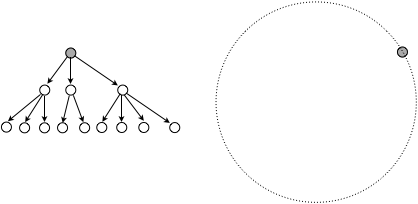
\includegraphics[scale=0.45]{FiguresGraph/TreeOutplanar1}
       \caption{Beginning an outerplanar drawing of a rooted tree $\t$: Placing $\t$'s root on a circle.}
  \label{fig:treeoutplanar1}
\end{center}
\end{figure}
\begin{figure}[hbt]
\begin{center}
       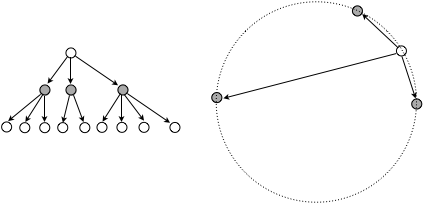
\includegraphics[scale=0.45]{FiguresGraph/TreeOutplanar2}
       \caption{Continuing an outerplanar drawing of $\t$.: Placing $\t$'s root's children around the circle}
  \label{fig:treeoutplanar2}
\end{center}
\end{figure}
The third figure depicts an entire outerplanar drawing of $\t$.
\begin{figure}[hbt]
\begin{center}
       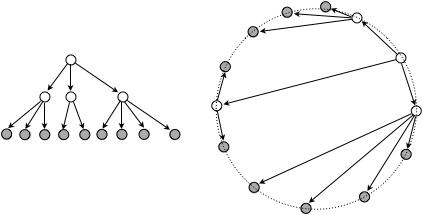
\includegraphics[scale=0.45]{FiguresGraph/TreeOutplanar3}
       \caption{A complete outerplanar drawing of $\t$.}
  \label{fig:treeoutplanar3}
\end{center}
\end{figure}

\begin{prop}
\label{thm:basic-outerplanar-stuff}
Let $\g$ be an outerplanar graph.  Then:

\smallskip

\noindent {\bf (a)}
$\g$ is planar.

\ignore{********
{\bf (b)} & $\g$ is a subgraph of a Hamiltonian graph. 
{\Denis I removed the second item since Hamiltonian has been shifted after this section.}\\
*********}

\smallskip

\noindent {\bf (b)}
Every subgraph of $\g$ is outerplanar.

\smallskip

\noindent {\bf (c)}
At least one of $\g$'s vertices has degree $\leq 2$.
\end{prop}

\begin{proof}
{\bf (a)}
$\g$'s planarity can be inferred from our ability to draw $\g$'s edges as noncrossing chords of the circle.

\medskip

\noindent {\bf (b)} 
We can produce a drawing of any subgraph  $\g'$ of $\g$ that witnesses $\g'$'s outerplanarity by erasing some vertices and/or some edges from our outerplanarity-witnessing drawing of $\g$.  These erasures cannot introduce any edge-crossings.

\medskip

\noindent {\bf (c)}
One verifies easily that part (c) holds for all outerplanar graphs having $\leq 3$ vertices.  Focus, therefore, on an arbitrary outerplanar graph $\g$ that has $> 3$ vertices.  Since adding more edges to a graph cannot decrease the degree of any vertex, we lose no generality by focusing on a graph $\g$ that is {\em maximally} outerplanar, in the sense that adding any new edge to $\g$ would destroy our ability to draw $\g$'s edges in a noncrossing manner.
\index{maximal outerplanar graph}

\smallskip

Because $\g$ has more than $3$ vertices, and because all of its vertices lie on a circle (in the drawing that witnesses $\g$'s outerplanarity), there must be pairs of vertices of $\g$ that are not adjacent along the circle.  Let $u$ and $v$ be nonadjacent (in the drawing) vertices of $\g$ such 
that the distance between $u$ and $v$ (measured in term of number of edges that one must traverse to reach one vertex from the other) is {\em minimal} among pairs of nonadjacent vertices.  We must consider two cases.
\begin{itemize}
\item
If the distance between $u$ and $v$ were {\em exactly} $2$, then the unique vertex that lies between $u$ and $v$ along the circle would have degree $2$.
\item
If the distance between $u$ and $v$ {\em exceeded} $2$, then there would be at least {\em two} vertices that lie between $u$ and $v$ in either direction around the circle.  But in this case, there would be two nonadjacent vertices that were closer to one another than $u$ and $v$---which contradicts our choice of $u$ and $v$ as a pair of {\em closest} nonadjacent vertices.
\end{itemize}
We conclude that $\g$ must have a vertex of degree $\leq 2$.  \qed
\end{proof}

\medskip

We return now to our primary concern---vertex-colorings in graphs.

\medskip

The $3$-vertex cycle $\cc_3$ witnesses the fact that not every outerplanar graph is $2$-colorable. Therefore, the chromatic number for the family of outerplanar graphs can be no smaller than $3$.  We now show that $3$ is, in fact, the chromatic number for this family.  Our inductive proof of this fact can easily be turned into an efficient $3$-coloring algorithm.

\begin{prop}[The $3$-Color Theorem for Outerplanar Graphs]
\label{thm:OP-3-colorability}
Every outerplanar graph is $3$-colorable.
\end{prop}

\begin{proof}
We proceed by induction on the number of vertices in the outerplanar graph to be colored.

\smallskip

\noindent {\sf Base case}.
We leave to the reader the task of finding $3$-colorings for small outerplanar graphs---say those having $\leq 3$ vertices.

\medskip

\noindent {\sf Inductive assumption}.
Assume that every outerplanar graph having $< n$ vertices is $3$-colorable.

\medskip

\noindent {\sf Inductive extension}.
Focus on an arbitrary $n$-vertex outerplanar graph $\g$.

\smallskip

\index{incident edges}

By Proposition~\ref{thm:basic-outerplanar-stuff}(d), $\g$ has a vertex $v$ of degree $\leq 2$.  Let us remove vertex $v$ from $\g$, along with its {\it incident} edges, i.e., those that connect $v$ to the rest of $\g$; call the resulting graph $\g'$.  Now: 
\begin{itemize}
\item
$\g'$ is clearly outerplanar.

\smallskip

This will be clear once we ``stitch'' together the circle that we ``damaged'' by removing $v$.
\item
$\g'$ has {\em fewer than} $n$ vertices.
\end{itemize}
By our inductive hypothesis, $\g$ is $3$-colorable.

\smallskip

But now we can reattach vertex $v$ to $\g'$ by replacing the edges that attach $v$ to $\g$. Moreover, we can now color $v$ using whichever of the $3$ colors on $\g$ that is {\em not} used for $v$'s neighbors in $\g$.  Once we so color $v$, we will have a $3$-coloring of $\g$.

\smallskip

Our induction is, thus extended, which completes the proof.  \qed
\end{proof}


\subsubsection{On vertex-coloring {\em planar} graphs}
\label{sec:planar-graphs}

 \index{planar graphs} \index{graph!planar}
 
The larger of this section's two graph families comprises {\it planar graphs}: graphs that can be drawn (on a two-dimensional medium) with no crossing edges.

\bigskip

\noindent \fbox{
\begin{minipage}{0.96\textwidth}
The historically original focus on planar graphs and their vertex-colorings stemmed from viewing the graphs as abstractions of geographical maps.  The political units on a map (countries and/or cities and/or \ldots) became the vertices of a graph $\g$.  And, political units that shared a border led to an edge connecting the corresponding vertices of $\g$.

\smallskip

Of course, every abstraction idealizes reality in some way.  In this geographical setting, the major idealization is the assumption that ``adjacent" units shared a boundary that had non-zero length.  Adjacencies such as one observes with the US states of Arizona, Utah, Colorado, and New Mexico---the famous ``four corners states"---which meet at a point were not allowed in the abstraction.

\smallskip

The chromatic number of $\g$ then became, quite literally, the numbers of shades of ink that one would need in order to print the map in a way that assigned different colors to units that shared a border.
\end{minipage}
}

\bigskip

\noindent
In a clique, every pair of vertices are mutually adjacent.  Therefore:

\smallskip

{\em For all $n$, the $n$-vertex clique $\k_n$ can be colored with $n$ colors but no fewer.}

\smallskip

\noindent
Thus, the $4$-vertex clique $\k_4$ witnesses the fact that {\em not every planar graph is $3$-colorable}.  But it also raised the question, {\em Is every planar graph $4$-colorable}?


\index{Appel, Kenneth}  \index{Haken, Wolfgang}

\paragraph{A. On the $4$-Color Theorem for planar graphs}

A century-plus attempt to prove that $4$ colors suffice for planar graphs culminated in one of the most fascinating dramas in modern mathematics:  American mathematicians Kenneth Appel and Wolfgang Haken enlisted the help of their families---{\em and of their computer!}---as they crafted a proof of their renowned {\it $4$-Color Theorem for Planar Graphs}.  Their 1974 proof was long enough to consume {\em two} journal articles---both appearing in volume 21 of the {\it Illinois Journal of Mathematics} \cite{AppelH77a,AppelH77b}.

\index{The $4$-Color Theorem for Planar Graphs}
\index{coloring planar graphs!the $4$-Color Theorem}

\begin{theorem}[The $4$-Color Theorem for Planar Graphs~\cite{AppelH77a,AppelH77b}]
\label{thm:Four-ColorTheorem}
Every planar graph is $4$-colorable.
\end{theorem}

\index{The $4$-Color Problem for planar graphs} 

The proof of Theorem~\ref{thm:Four-ColorTheorem} is beyond the scope of any textbook, even an advanced one, but the backstory of the proof is truly fascinating!  And, the backstory supplies ample motivation for the proofs we present of the $6$-color and $5$-color analogues of the Theorem.

\medskip

Beginning with a failed attempt in 1875 to prove that every planar map can be $4$-colored, the so-called {\it $4$-Color Problem} held the world of discrete  mathematics in thrall for roughly a century before Appel and Haken announced their proof of Theorem~\ref{thm:Four-ColorTheorem} in 1974.  But, this proof notwithstanding, the drama surrounding the $4$-Color Problem persisted, because of the Appel-Haken proof's reliance---in a fundamental way---on a computer program that checked more than a thousand essential, but clerical, assertions (about forbidden subgraphs).  It took the
mathematics community years before the Appel-Haken proof, with its massive complexity and unprecedented employment of ``collaboration'' by computer, was generally accepted.

\smallskip

Even readers who might be daunted by the primary references \cite{AppelH77a,AppelH77b} that accompany our statement of the Theorem may well enjoy the much more accessible articles \cite{AppelH77c,AppelH89} in which the authors summarize---and, at a rather sophisticated level, popularize---this marvelous mathematical tale.

\bigskip

We turn now to the eminently accessible proofs of the $6$- and $5$-color analogues of Theorem~\ref{thm:Four-ColorTheorem}.  There are significant lessons within the proofs of these 
analogues.
\begin{itemize}
\item
The weaker, $6$-color, version of the Theorem can be proved in much the same way as its
outerplanar-graph cousin, Proposition~\ref{thm:OP-3-colorability}.  We
present this proof in detail in Paragraph B.  
\item
The proof of the stronger, $5$-color, version of the Theorem already requires us to break the world into multiple cases---but only a single-digit number of cases, in contrast to the four-digit list of cases engendered by the proof of Theorem \cite{AppelH77a,AppelH77b}.  That said, the complexity of the $5$-color theorem has led us to include its proof only as an ``Enrichment Topic''; see Paragraph C.
\end{itemize}


\paragraph {B. The $6$-Color Theorem for planar graphs}

The first step in showing that every planar graph can be vertex-colored using $6$ colors resides in the following analogue for planar graphs of Proposition~\ref{thm:basic-outerplanar-stuff}(d), which asserts that every outerplanar graph has a vertex of degree $2$.

\begin{lemma}
\label{thm:PlanarGraph-degree5}
Every planar graph has a vertex of degree $\leq 5$.
\end{lemma}

\index{graph!planar!face in a drawing} \index{planar graph!face in a drawing} 

\begin{proof} {\em (Lemma~\ref{thm:PlanarGraph-degree5})}
Let us focus on a planar drawing of a (perforce) planar graph $\g$ which has $n$ vertices, $e$ edges, and $f$ {\it faces}.  A {\it face} in a drawing of $\g$ is a polygon whose sides are edges of
$\g$, whose points are vertices of $\g$, and whose interiors are ``empty"---no edge of $\g$ crosses through a face.

\bigskip

\noindent \fbox{
\begin{minipage}{0.96\textwidth}
Now that we know about faces, we can finally describe the origin of the term {\it outerplanar}.  A graph $\g$ is outerplanar if it can be drawn (on a $2$-dimensional medium) in the following manner.  All of $\g$'s vertices are placed around a circle, and all of $\g$'s edges are drawn as noncrossing chords of the circle.  The region outside the vertex-bearing circle is, thus, the {\em outer} face of this special planar drawing of $\g$.
\end{minipage}
}
\bigskip

The following auxiliary result derives a celebrated ``formula'' attributed to Euler.

\index{Euler, Leonhard} \index{Euler's Formula}

\begin{prop} [Euler's Formula for Planar Graphs]
\label{thm:Euler-Formula}
Given the indicated drawing of $\g$, we have
\begin{equation}
\label{eqn:Eulers-formula}
n \ - \ e \ + \ f \ \ = \ \ 2
\end{equation}
\end{prop}

\medskip

We defer proving Proposition~\ref{thm:Euler-Formula} so that we can proceed with our ongoing proof of Lemma~\ref{thm:PlanarGraph-degree5}.  We devote Subsection~\ref{subsec:validationEulerFormula} to two quite different proofs of Euler's formula.

\medskip

\index{graph!planar!maximal}

As we approach the next step in the proof of Lemma~\ref{thm:PlanarGraph-degree5}, we  simplify the setting by assuming henceforth that $\g$ is {\em connected} and that it is a {\em maximal} planar graph---meaning that one cannot add any new edge to the drawing without crossing an existing edge (and, thereby, destroying planarity).  Fig.~\ref{fig:K5andK3by3} illustrates the notion 
of maximality by providing planar drawings of two connected {\em maximal} planar graphs.
\begin{figure}[hbt]
\begin{center}
       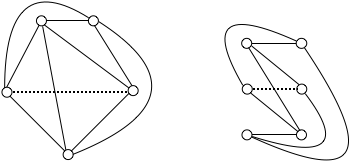
\includegraphics[scale=0.55]{FiguresGraph/K5andK3by3}
\caption{Maximal planar drawings of $\k_5$ (left) and $\k_{3,3}$ (right).  The reader cannot add an edge to either drawing without destroying planarity---i.e., without introducing any crossing edges.  For reference, we use dotted lines in the figure to exhibit the extra edges that would augment the depicted planar graphs to the (inherently nonplanar) graphs $\k_5$ (on the left) and $\k_{3,3}$ (on the right).}
  \label{fig:K5andK3by3}
\end{center}
\end{figure}
The assumption of maximality only strengthen's the Lemma's conclusion by (apparently) making it more difficult to find a small-degree vertex.

\ignore{**********
{\Denis I don't think the notion of maximality is simple, may be we should add a figure here?}
{\Arny The notion certainly helps ME to think about the proof ... but I am probably not
a typical reader, right?  I think that a figure would be very good here.  Maybe it would suffice to
"challenge" the reader to add one more edge to a planar drawing of $\k_5$ or of $\k_{3,3}$ -- or
of both!!}
***********}

\smallskip

With the maximality assumption in place, we now adapt a pedagogical tool from \cite{Berge73}, in order to make the following counting argument easier to follow.  We construct a {\em directed bipartite} graph {\bf G} which exposes certain features of $\g$'s structure.  On one side of {\bf G} are the $f$ faces of $\g$; on the other side are $\g$'s $e$ edges.  {\bf G} contains an arc from each face of $\g$ to each edge of $\g$ that forms a ``side'' of the polygonal drawing of the face.  Because $\g$ is a {\em maximal} planar graph, we have:
\begin{itemize}
\item
Each face of $\g$ is a $3$-cycle, hence involves three vertices.
\item
Each edge of $\g$ touches two faces.
\item
Each edge of $\g$ touches two vertices.
\end{itemize}

Let us now put these facts together, and assume, for contradiction, that every vertex of $\g$ had degree $\geq 6$.  We would then find that
\[ \left[ f \ \ \leq \ \ \frac{2}{3} e \right] \ \ \ \ \mbox{ and } \ \ \ \ \Big[ e \ \ \geq \ \ 3n \Big] \]
Incorporating these two bounds into Euler's Formula (\ref{eqn:Eulers-formula}), we arrive at the following contradiction.
\[ 2 \ \ = \ \ n \ - \ e \  + \ f \ \ \leq \ \ \frac{1}{3} e \ - \ e \ + \ \frac{2}{3} e \ \ = \ \ 0 \]
This contradiction proves that every planar graph must have a vertex of degree $\leq 5$.
 \qed-Lemma~\ref{thm:PlanarGraph-degree5}
\end{proof}

\medskip

We finally have the tools to color any planar graph using $6$ colors.

\index{The $6$-Color Theorem for Planar Graphs}
\index{coloring planar graphs!the $6$-Color Theorem}

\begin{prop}[The $6$-Color Theorem for Planar Graphs]
\label{thm:P-6-colorability}
Every planar graph is $6$-colorable.
\end{prop}

\begin{proof}
The $2$-Color Theorem for Outerplanar Graphs (Proposition~\ref{thm:OP-3-colorability}) and this result follow via almost-identical inductions on the number of vertices in the graph $\g$ that is being colored.  Both arguments:
\begin{enumerate}
\item
remark that the target number of colors is adequate for small graphs

\smallskip

For outerplanar graphs, ``small'' means ``$\leq 3$ vertices''.  For planar graphs, it means ``$\leq 4$ vertices''.

\item
remove from $\g$ a vertex $v$ of smallest degree $d_v$, together with all incident edges

\smallskip

For outerplanar graphs, we guarantee that $d_v \leq 2$ (Proposition~\ref{thm:basic-outerplanar-stuff}(d)).  For planar graphs, we guarantee that $d_v \leq 5$ (Lemma~\ref{thm:PlanarGraph-degree5}).

\item
inductively color the vertices of the graph left after the removal of $v$

\smallskip

Let us denote by $\g'$ the graph obtained by removing $v$ from $\g$.  Then: 

For outerplanar graphs, we color $\g'$ with $\leq 3$ colors (Proposition~\ref{thm:OP-3-colorability}).  For planar graphs, we use an inductive assumption that $\g'$ can be colored with $\leq 6$ colors. 

\item
reattach $v$ via its $d_v$ edges and then color $v$.

\smallskip

Note that the coloring guarantee in both results---Proposition~\ref{thm:OP-3-colorability} for outerplanar graphs and the current result for planar graphs---allows us to use $d_v +1$ colors to color $\g$.  Because $v$ has degree $d_v$, it can have no more than $d_v$ neighboring vertices in $\g'$, so our access to $d_v +1$ colors guarantees that we can successfully color $v$.
\end{enumerate}
The proofs of the $3$-colorability of outerplanar graphs and the $6$-colorability of planar graphs thus differ only in the value of $d_v$.  \qed
\end{proof}


\paragraph{C. $\oplus$ The $5$-Color Theorem for planar graphs}
\index{The $5$-Color Theorem for Planar Graphs}
\index{coloring planar graphs!the $5$-Color Theorem}

\begin{prop}[The $5$-Color Theorem for Planar Graphs]
\label{thm:5colors}
\label{thm:P-5-colorability}
Every planar graph is $5$-colorable.   \cite{Heawood90}
\end{prop}

\bigskip

%The proof, being rather technical, is relegated to the Appendix, as Chapter~\ref{Appendix:5colors}.

\noindent \fbox{
\begin{minipage}{0.96\textwidth}
The case analysis in the following proof is a bit more complex than in most of the results in the text, but a methodical reading should make the proof accessible to the reader.  Moreover,  the {\em roadmap} of the case analysis is a valuable lesson in how mathematics is really done!

\smallskip

The motivated reader will be able to recast the totally positive proof we present into the form of a proof by contradiction.  The positive version should be more to the taste of a computation-oriented reader---but both proofs are equally correct.
\end{minipage}
}

\ignore{*************
The proof again (I mean like for 6 colors) is by recurrence but we add
here a contradiction argument:
Similarly, we focus on a vertex with degree 5 (at some points, we will
have to justify this)
This vertex (call it x) has 5 neighbors
The problem is when they are colored by the 5 colors, otherwise it is
colored by a missing one.
Let now label these 5 vertices from 1 to 5.
Consider the vertices 1 and 3, colored by two different colors and the
sub-graph composed of vertices with colors 1 and 3
If these two vertices are in disjoint connected components, (case 1), it is
easy to color x by reverting the colors 1 and 3 in one component
(see figure)
Thus, the problem is when there exists an alternate path (in term of
colors) between vertex 1 and vertex 3
in this case (case 2), consider vertices 2 and 4, using a similar process
as in case 1, if there are two connected components
we are done (x can be colored by reverting the colors along the path
in one component), otherwise, there is an alternate path
between 2 and 4.
However, since the graph is planar, then, both alternate paths will
intersect, which is impossible
************************}

\begin{proof}
We henceforth discuss, without explicit mention, only {\em valid} vertex-colorings---in which neighboring vertices get different colors.  We proceed by induction.

\medskip

\noindent {\sf Base case.}
Because the $5$-clique $\k_5$ is obviously $5$-colorable, so also must be all graphs having $\leq 5$ vertices.  Therefore, we know that any non-$5$-colorable graph would have $\geq 6$ vertices.

\medskip

\noindent {\sf Inductive hypothesis.}
Assume, for induction, that every planar graph having $\leq n$ vertices is $5$-colorable.

\medskip

\noindent {\sf Inductive extension.}
If the proposition were false, then there would exist a planar graph $\g$ having $n+1$ vertices which is not $5$-colorable.  By Lemma~\ref{thm:PlanarGraph-degree5}, $\g$ would have a vertex $v$ of degree $\leq 5$.  The remainder of the proof focuses on the graph $\g$, its minimal-degree vertex $v$, and on $v$'s $(d_v \leq 5)$ neighbors in $\g$.

\smallskip

If there were a coloring of $\g$'s vertices in which $\leq 4$ colors were used to color $v$'s neighbors, then the following analogue of the coloring strategy of Proposition~\ref{thm:P-6-colorability} would produce a $5$-coloring of $\g$.
\begin{enumerate}
\item
Remove vertex $v$ and its incident edges from $\g$, thereby producing the $n$-vertex planar graph $\g'$.
\item
Produce a $5$-coloring of $\g'$ that uses only $4$ colors for the vertices that are neighbors of $v$ in $\g$.
\item
($a$) Reattach vertex $v$ and its edges to $\g'$, thereby reconstituting $\g$.

\smallskip

($b$) Color $v$ with whichever of the $5$ available colors is not used to color $v$'s neighbors.
\end{enumerate}

\smallskip

In order to proceed in pursuit of a contradiction, we must understand what structural features of $\g$ make it impossible to use only $4$ colors on $v$'s neighbors when $5$-coloring $\g$.  There are three important situations to recognize.
\begin{description}
\item[{\sf Case 1}.]
Vertex $v$ has degree $\leq 4$.

\smallskip

By definition, $\leq 4$ colors are used to color $v$'s neighbors in this case.
\end{description}
Note that, in all remaining cases, vertex $v$ has precisely $5$ neighbors---or else, we would have invoked Case 1 to color $\g$ with $5$ colors.
\begin{description}
\item[{\sf Case 2}.]
For some $5$-coloring of $\g$, $\geq 2$ neighbors of $v$ get the same color.

\smallskip

Because $v$ has exactly $5$ neighbors, in this case, only $4$ colors are used to color these neighbors.
\end{description}
In all remaining cases, the $5$ neighbors of $v$ receive distinct colors.
\begin{description}
\item[{\sf Case 3}.]
For some $5$-coloring of $\g$, some two neighbors of $v$---call them $v_1$ and $v_2$---reside in distinct components of $\g$ once $v$ and its incident edges are removed from $\g$.

\smallskip

As before, let $\g'$ be the (in this case, disconnected) graph that results when $v$ and its incident edges are removed from $\g$.  For $i = 1,2$ Let $\g_i$ be the component of $\g'$ that contains vertex $v_i$.

Say that, under the $5$-coloring of $\g$ that we are focusing on, $v_1$ is colored {\it red} and $v_2$ is colored {\it green}.

\smallskip

Let us recolor the vertices of $\g_1$ so that vertex $v_1$ is now colored {\it green}.  (One needs only switch the colors {\it red} and {\it green} in the existing coloring of $\g_1$ to achieve this.)  It is always possible to do this in a way that does not affect the valid coloring of $\g_2$ because $\g_1$ and $\g_2$ are mutually disjoint.

\smallskip

Once we have thus-recolored $\g_1$, we have a $5$-coloring of $\g$ for which Case 2 holds.  (In fact, we can color vertex $v$ {\em red} when we reattach it to $\g'$.)
\end{description}

\smallskip

\noindent
We now see that Cases 1--3 cannot prevent us from $5$-coloring $\g$, so we are left with the following minimally constrained situation.
\begin{description}
\item[{\sf Case 4}.]
\begin{itemize}
\item
Every minimum-degree vertex of $\g$ has $5$ neighbors.

\smallskip

For the minimum-degree vertex $v$, let us call these neighbors $v_1$, $v_2$, $v_3$, $v_4$, $v_5$, {\em in clockwise order within the planar drawing}.
\item
In every $5$-coloring of $\g$, the neighbors of every minimum-degree vertex receive distinct colors.

\smallskip

For vertex $v$, let us say that neighbor $v_i$ receives color $c_i$.
\end{itemize}
The leftmost graph in 

****************************
FIGURE 1 
{Denis Put right ref here}
***************************

depicts the portion of $\g$ comprising vertex $v$ and its neighbors.  In the figure, we use integer $i$ to denote, ambiguously, vertex $v_i$ and its assigned color $c_i$.  The question mark ``?'' that ``colors'' vertex $v$ indicates that we do not yet know what color to assign to $v$.  The other two graphs in the figure depict schematically how we have dealt with Case 3 above.
\begin{itemize}
\item
All neighbors of vertex $v$ remain in the same component of $\g$ when $v$ and its incident edges are removed.
\end{itemize}
\end{description}
To analyze Case 4, we focus on vertices $v_1$ and $v_3$ in

*******************************
 FIGURE 1.
{Denis Put right ref here}
*********************************

Importantly, these vertices have received distinct colors ($c_1$ and $c_3 \neq c_1$, respectively), and these vertices are not adjacent to one another as one makes a clockwise sweep around vertex $v$.

\smallskip

Now take $\g$ and focus only on the vertices that are colored $c_1$ or $c_3$ (as are $v_1$ and $v_3$, respectively) and on the vertices that are colored $c_2$ or $c_4$ (as are $v_2$ and $v_4$, respectively).  One sees from Figure 2 that:
\begin{itemize}
\item
$\g$ can---{\em but need not}---contain a path whose vertices alternate  colors $c_1$ and $c_3$. Call this a ``$c_1$-$c_3$ path'' between vertices $v_1$ and $v_3$.
\item
$\g$ can---{\em but need not}---contain a path whose vertices alternate colors $c_2$ and $c_4$.  Call this a ``$c_2$-$c_4$ path'' between vertices $v_2$ and $v_4$.
\item
$\g$ {\em cannot} contain both of the paths just described, i.e., a $c_1$-$c_3$ path between $v_1$ and $v_3$ {\em and} a $c_2$-$c_4$ path between $v_2$ and $v_4$.

\smallskip

{\em These two paths, if they existed, would cross one another---which is forbidden because $\g$ is a {\em planar} graph.}  See Figure 2.

*************************
Denis, references
*************************

\end{itemize}
It follows that {\em either} $\g$ does not contain a $c_1$-$c_3$ path between $v_1$ and $v_3$ {\em or} $\g$ does not contain a $c_2$-$c_4$ path between $v_2$ and $v_4$.  Say, with no loss of generality, that the former path does not exist.  Then we can switch colors $c_1$ and $c_3$ beginning with vertex $v_1$ and obtain a coloring of $\g$ in which $v_1$ and $v_3$ both receive the color $c_3$.  We can then proceed as in Case 2 to get a $5$-coloring of $\g$.

\smallskip

This four-case analysis shows that we can always produce a $5$-coloring of $\g$, which completes the proof.  \qed
\end{proof}

\bigskip

We close our study of vertex-colorings of planar graphs with an overview of the intellectual cost-benefit tradeoff that we have exposed:
\begin{itemize}
\item
A straightforward recursive coloring strategy suffices if one is willing to settle for a $6$-color palette when coloring planar graphs (Proposition~\ref{thm:P-6-colorability}).
\item
A four-case analysis, in which one case comprises several subcases, is needed in order to eliminate one of the colors from our palette, i.e., to achieve a $5$-coloring strategy (Proposition~\ref{thm:5colors}).
\item
An analysis involving close to 2000 cases is needed in order to achieve the provable optimal, a $4$-color palette that always works (Theorem~\ref{thm:Four-ColorTheorem}).
\end{itemize}

\subsubsection{Two validations of Euler's Formula}
\label{subsec:validationEulerFormula}
\index{Euler's Formula}

We now develop two quite different proofs of Proposition~\ref{thm:Euler-Formula}, which expose different ways to think about the identity.

\medskip

\index{Euler's Formula!validation via structural induction}

\noindent {\bf Validation via structural induction}. 
Our first approach validates (\ref{eqn:Eulers-formula}) by growing a planar graph $\g$
inductively, edge by edge.  Note that we formulate our induction a bit differently than our earlier, simpler ones, particularly in the Inductive hypothesis.

\smallskip

\noindent {\sf Base case}.
The Formula clearly holds for the smallest planar graphs, including the smallest interesting one, $\cc_3$, which has $n = e = 3$ and $f =2$ (the inner and outer faces of the ``triangle'').

\smallskip

\noindent {\sf Inductive hypothesis}.
Assume that the Formula holds for a given graph $\g$.

\smallskip

\noindent {\sf Inductive extension}.
We extend our induction by growing the current version of $\g$, by adding a new edge.  Two cases arise.
\begin{itemize}
\item
{\it The new edge connects existing vertices.}
In this case, this augmentation of $\g$ increases the number of edges ($e$) and the number of faces ($f$) by $1$ each, while keeping the number of vertices ($n$) unchanged.

\item
{\it The new edge adds a new vertex, which is appended to preexisting vertex.}
In this case, this augmentation of $\g$ keeps the number of faces ($f$) unchanged while
it increases by $1$ both the number of edges ($e$) and the number of vertices ($n$). 
\end{itemize}
In both cases Euler's Formula (\ref{eqn:Eulers-formula}) continues to hold as we augment $\g$.  

The augmentation thus extends the induction, hence validates the Formula.  \qed

\bigskip

\index{Euler's Formula!validation via deconstruction}

\noindent {\bf Validation via deconstruction}.
Let us be given a planar graph $\g$ that has $n$ vertices, $e$ edges, and $f$ faces.  We validate Formula (\ref{eqn:Eulers-formula}) by deconstructing $\g$ and showing that each step in the process preserves as {\it invariant} the expression
\begin{equation}
\label{eq:phi-in-euler-formula}
 \phi(n,e,f) \ = \ n-e+f
\end{equation}

\bigskip

\index{invariants}
\noindent \fbox{
\begin{minipage}{0.96\textwidth}
\textit{Invariants} are extremely important conceptual tools when crafting proofs.  The idea underlying their use is to find an expression $\phi(\circ)$ whose value is preserved---i.e., it ``holds
invariant"---as some relevant process proceeds.

\smallskip

With many mathematical concepts---including the notion of invariant---it is easier to grasp the concept by experiencing examples than by internalizing abstract explanations.  Therefore, we recommend that the reader follow this second validation of Euler's Formula while keeping track of the invariance of expression $\phi(n,e,f)$ of (\ref{eq:phi-in-euler-formula}).
\end{minipage}
}
\bigskip

\noindent
Focus on the following two-phase process.
\begin{description}
\item[{\bf Phase 1}.]
Iterate the process of removing edges from $\g$ until some edge-removal reduces $\g$ to a graph with a single face.

\smallskip

The reader should verify that this termination condition is equivalent to stopping when the remaining graph is a (connected) tree.

\medskip

{\sf The action}.
If the graph remaining at some step contains an edge that is shared by two distinct faces, then remove any such edge.

\smallskip

Fig.~\ref{fig:planarStep1} illustrates Phase 1 for a (residual) graph having $n=8$ vertices, $e=11$ edges, and $f=5$ faces.
\begin{figure}[hbt]
\begin{center}
   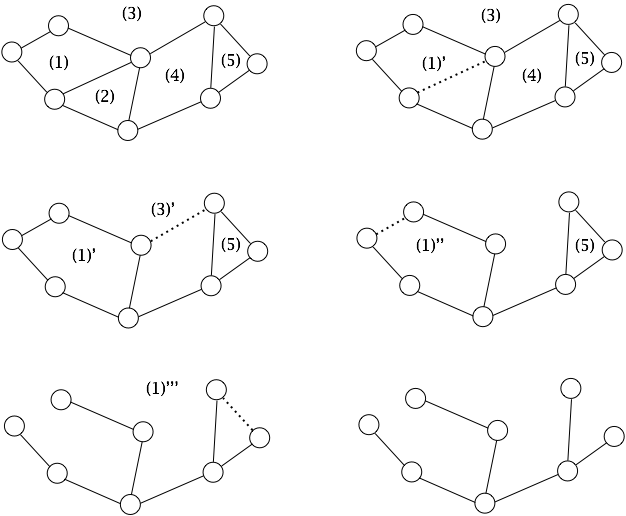
\includegraphics[scale=0.35]{FiguresGraph/planarStep1}
\caption{Illustrating Phase 1: From top left to bottom right, each transformation preserves the invariant $\phi(n,e,f)$.  The first transformation removes the edge shared by faces (1) and (2), creating a new, merged, face (1)'.}
  \label{fig:planarStep1}
\end{center}
\end{figure}

\medskip

{\sf The analysis}.
\begin{itemize}
\item
The graph remaining after an edge-removal is still planar, so we can continue the process.
\item
The process preserves the value of function $\phi$; i.e.,
\[ \phi(n,e,f) \ = \ \phi(n,e-1,f-1) \]
This is because $n$ is unchanged, while $e$ and $f$ are each reduced by $1$.
\end{itemize}

\item[{\bf Phase 2}.]
Iterate the following process of removing vertices from the tree produced by Phase 1, until only one vertex remains.

\medskip

{\sf The action}.
Remove any leaf of the current tree, together with its incident edge.

\smallskip

Fig.~\ref{fig:planarStep2} illustrates the action of Phase  2 for a tree having $n=8$ vertices---hence, $e=7$ edges and $f=1$ face.
\begin{figure}[hbt]
\begin{center}
   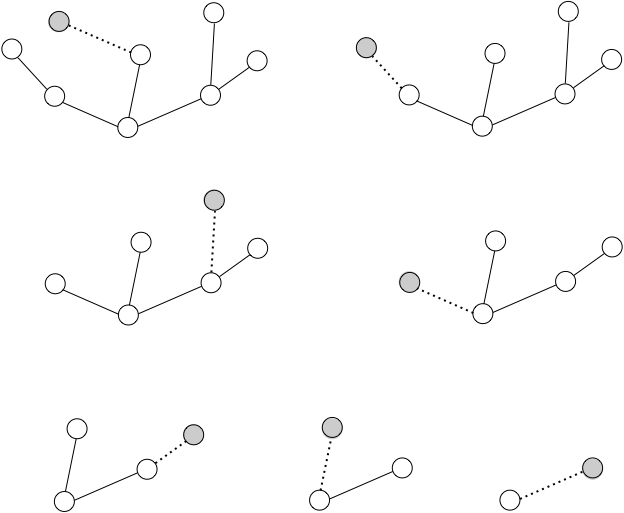
\includegraphics[scale=0.35]{FiguresGraph/planarStep2}
 \caption{Illustrating Phase 2: We remove a sequence of leaves, each with its incident edge, until we reach a single vertex.  Here again, $\phi$ remains invariant after each leaf-removal.}
  \label{fig:planarStep2}
\end{center}
\end{figure}

\medskip

{\sf The analysis}.
The value of $\phi$ remains invariant under each leaf-removal:
\[ \phi(n,e,f) \ = \ \phi(n-1,e-1,f) \]
To wit, $f$ is unchanged ($f \equiv 1$ for a tree), while $n$ and $e$ are each reduced by $1$.
\end{description}

\medskip

\noindent {\sf The cumulative analysis}.
\begin{itemize}
\item
The described process executes a number of steps exactly equal to the number of edges of the graph $\g$ that we begin with.  Specifically, the edge-removing Phase 1 removes $e-n$ edges, while the leaf-removing Phase 2 removes $n-1$ vertices.
\item
At the end of the process, $e=0$ and $n=f=1$, so that the residual value of $\phi$ is $2$.  Because each action prescribed by the process preserves the value of $\phi$, we know that $\phi$ has the value $2$ also {\em before} each edge-removal and leaf-removal.
\end{itemize}
We conclude, in summation, that at the start of the process, $\phi(n,e,f)$ had the value $2$.  In other words, $n-e+f = 2$, as asserted by Euler's Formula.   \qed

\bigskip

\noindent \fbox{
\begin{minipage}{0.96\textwidth}
Our study of vertex-coloring in graphs has focused almost entirely on planar and outerplanar graphs.  This is because---aside from the importance of such graphs in applications---their vertex-coloring problems can be studied entirely in terms of the mathematical structure of the graphs being colored.  Vertex-coloring for broader families of graphs usually cannot be studied solely by focusing on the target graph's structure:  Algorithmic issues arise quite early in the coloring process (although of course, mathematics is employed to analyze the algorithms).

\smallskip

In closing our treatment of this topic, though, we remark that there are many interesting algorithmic problems relating to vertex-coloring arbitrary graphs.  The following such result dates to the earliest days of the study of {\sf NP}-completeness \cite{GareyJ79,Karp72}.

\smallskip

\hspace*{.075in}
{\em For any fixed $k \geq 3$, the problem ``Is graph $\g$ $k$-colorable" is {\sf NP}-complete}.

\smallskip

This complexity-theoretic result suggests that {\em optimal} vertex-coloring is computationally inherently difficult.  The ``sting" of the result is moderated by the existence of ``greedy'', hence efficient, vertex-coloring algorithms that give quite good results in practice \cite{CLRS}.  The term ``greedy" here refers to algorithms that allocate a yet-unused color to a vertex only when no uncolored vertex can be validly colored with an already-used color.  (See Footnote~\ref{foot:greedy} in Chapter~\ref{ch:Graphs1}.)
\end{minipage}
}


\section{Path and Cycle Discovery Problems in Graphs}
\label{sec:path-cycle-problems}

Just as various genres of {\it spanning trees} are used to ``summarize'' aspects of the {\em connectivity} structure of a  graph $\g$, various genres of {\it paths} and {\it cycles} in $\g$ are often useful to ``summarize'' aspects of $\g$'s {\em traversal} structure.  This section is devoted to a range of problems related to determining the existence in a graph $\g$ of a path or a cycle that {\em completely} ``summarizes'' $\g$'s traversal structure---either by containing every edge of $\g$ precisely once (the {\it Eulerian} version of ``traversal summarization") or by containing every vertex of $\g$ precisely once (the {\it Hamiltonian} version of ``traversal summarization").

We generally focus in this section only on {\em undirected} paths and cycles in {\em undirected}, {\em unweighted} graphs.  Extending the notions we discuss to their directed analogues in directed and/or weighted graphs, will be accomplished via carefully crafted exercises.  In a similar, but simpler, vein, we generally discuss only problems concerning {\em cycles}, leaving to the reader the analogous path-related notion.  We begin by delimiting the two main classes of cycle-discovery problems that we study.

\bigskip

\index{graph!Eulerian cycle} \index{Eulerian cycle}
\index{graph!Eulerian circuit} \index{Eulerian circuit}  \index{Euler, Leonhard}

{\it Eulerian cycles (or, tours)}.
A cycle in a graph $\g$ that traverses each of $\g$'s {\em edges} precisely once is called an {\it Eulerian cycle} (or, often, an {\it Eulerian circuit}).  The edge-exhausting cycles/circuits/tours referred to by these several names were introduced as a topic of study in 1736 by the Swiss mathematician Leonhard Euler, whose name we have already encountered multiple times.  Euler allegedly identified the topic while contemplating how to devise a tour of the town of K\"{o}nigsberg that would cross each of the town's bridges precisely once.  The quest for Eulerian cycles in graphs is certainly one of the oldest problems---perhaps literally the oldest problem---in the fields now called {\it operations research} and {\it graph theory}.  (An edge-exhausting {\em path} in $\g$ is referred to in the obvious analogous way.)  When one views an Eulerian cycle as a ``map'' for traversing a graph---as did Euler when contemplating this problem---one often calls the cycle an {\it Eulerian tour}.  Traditionally, a graph that admits an Eulerian cycle is said to be {\it Eulerian}. 
 \index{graph!Eulerian tour} \index{Eulerian tour}  \index{graph!Eulerian} \index{Eulerian graph}

\medskip

\index{graph!Hamiltonian cycle} \index{Hamiltonian cycle}
\index{graph!Hamiltonian circuit} \index{Hamiltonian circuit}
\index{Hamilton, William Rowan} \index{Kirkman, Thomas Pennington}

{\it Hamiltonian cycles (or circuits, or tours)}.
A cycle in a graph $\g$ that encounters each of $\g$'s {\em vertices} precisely once is called a {\it Hamiltonian cycle}, (or, often, a {\it Hamiltonian circuit}).  This cycle-discovery problem is named in honor of the British mathematician Sir William Rowan Hamilton, who is credited with inventing the
concept in the mid-19th century.  (In fact, Hamilton's work on his eponymous cycles was anticipated by many decades in the work of fellow British mathematician, Thomas Pennington Kirkman.)  When one views a Hamiltonian cycle as a ``map'' for traversing a graph, one often calls the cycle a {\it Hamiltonian tour}.  Traditionally, a graph that admits a Hamiltonian cycle is said to be {\it Hamiltonian}.  (A vertex-exhausting {\em path} in a graph is referred to in the obvious analogous way.)  
 \index{graph!Hamiltonian tour}\index{Hamiltonian tour} \index{graph!Hamiltonian} \index{Hamiltonian graph}

\bigskip

Despite the conceptual duality between the edge-exhausting goal that underlies Eulerian paths/cycles and the vertex-exhausting goal that underlies Hamiltonian paths/cycles, these two graph-traversing goals differ from one another in virtually every significant mathematical and algorithmic respect.  It is rather easy to characterize the family of graphs that admit Eulerian tours and to find such a tour if it exists (Section~\ref{sec:EulerianCycle}); in sharp contrast, there is no known characterization of the family of graphs that admit Hamiltonian tours, and the computational problem of efficiently determining whether a graph admits such a tour is one of the major classical problems in the field of computational complexity  (Section~\ref{sec:Hamiltonian-cycle}).

%%%%%%%%%%%%%%%%%%%%%%%%%%%%%%%%%%%%%%%%%%%%%%%%%%%%

\subsection{Eulerian Cycles and Paths}
\label{sec:EulerianCycle}

The main results in this section characterize the families of directed and undirected graphs
that admit {\it Eulerian cycles} or {\it Eulerian paths}.  The proofs of these characterizations are
constructive: they consist of algorithms that efficiently find such a cycle or such a path when 
one exists.  We focus on graphs that are connected---but the algorithms we present can actually be 
adapted to find an Eulerian cycle or an Eulerian path in each connected component of a general
graph.

As we embark on our adventure, we note the following amusing fact: \\
{\em The problem of finding an Eulerian cycle in a graph $\g$ is
equivalent to the problem of drawing $\g$ ``cyclically"---i.e., while
starting and ending with the same vertex---without ever lifting one's
pencil.} \index{graph!drawing without lifting pencil}

\medskip

In the next two propositions, we develop---for both cycles and paths, in both undirected and
directed graphs---simple, elegant characterizations of graphs that admit Eulerian cycles and paths.
These characterization are validated via simple and efficient algorithms that determine
whether a given graph admits such a path or such a cycle.  To avoid ``special cases" that
disrupt the flow of a proof, let us restrict attention to graphs and digraphs that are {\em nontrivial}
in the sense that
\begin{itemize}
\item
each (di)graph has at least three vertices;
\item
each (di)graph is connected.
\end{itemize}
Within this domain, we have the following characterizations.

\begin{prop}[Eulerian Cycles]
\label{thm:eulerian-cycle}
{\bf (a)}
A connected undirected graph $\g$ admits an Eulerian cycle if, and only if,
every vertex of $\g$ has even degree.

{\bf (b)}
A connected directed graph $\g$ admits a directed Eulerian cycle if, and only if,
$\mbox{\sc indegree}(v) \ = \ \mbox{\sc outdegree}(v)$ for every vertex $v$ of $\g$.
\end{prop}

\ignore{*********
{\Denis The question of edge multiplicity should be addressed somewhere since in particular
the chinese postman is based on edge duplicates...}
{\Arny I do not understand what you are proposing.  If multiple edges occur just in one special
environment, then M. Occam tells us to introduce that complication JUST in that environment,
using the simpler more general situation in the body of the text.  We should discuss}
{\Denis right, my concern was on the basis of the induction proof...}
**********}

\begin{proof}
{\em Necessity.}
The conditions asserted in parts {\bf (a)} and {\bf (b)} are {\em necessary} because of
the following fact.  Every time any cycle traverses a vertex $v$ of a (di)graph $\g$, that 
encounter accounts for {\em two} edges that are incident to $v$: the cycle must ``enter'' $v$
using one edge and ``exit'' $v$ using a different edge.  (By assumption, the degenerate case 
of a (di)graph having just one vertex is not relevant here.)

\ignore{**********
{\Arny The original conditions were wrong.  An unconnected
graph CAN have an Eulerian cycle of the type we define, since we do not demand that 
the cycle contains all vertices.  Thus, by our definition, an Eulerian graph remains Eulerian 
if we add isolated vertices to it.  We must discuss this -- should we demand that the cycle
touches all vertices??}
{\Denis yes, for me, an eulerian cycle should touch all the vertices, I don't see any problem 
as we assumed that the graph is connected...}
************}

\medskip

\noindent {\em Sufficiency.} 
We now verify that Proposition's conditions are also {\em sufficient}.  We provide 
a complete proof of sufficiency only for part {\bf (a)} of the Proposition; we 
provide only hints regarding the sufficiency of the conditions in part {\bf (b)}.

\smallskip

We have a choice of proving sufficiency either by induction on the number of vertices in a 
graph or by induction on the number of edges in the graph.  While we invite the reader to 
develop the vertex-based proof, we focus only on the technically more streamlined edge-based proof. 

\smallskip

\ignore{**************
\begin{itemize}
\item
{\it For {\em undirected} graphs:} We note that $2$-vertex graphs
cannot have even vertex-degrees---and, indeed, as promised by the
Proposition, they cannot be Eulerian.  One can exhaustively enumerate
all $3$-vertex and $4$-vertex graphs and verify that the Proposition correctly
separates the ones that are Eulerian from those that are not.
\item
Focusing on {\em directed} graphs: We note that $2$-vertex digraphs can be
Eulerian---as witnessed by the $2$-vertex digraph each of whose vertices
hosts a single arc that points to the other vertex.  Once again, one can
perform an exhaustive enumeration of $3$-vertex and $4$-vertex digraphs
and verify that the Proposition correctly separates the Eulerian ones
from the non-Eulerian ones.
\end{itemize}
******************} 

\smallskip

Focus on a connected undirected graph $\g$ that has $m$ edges and $n$ vertices, each
vertex having nonzero even degree.  We prove by induction on $m$ that $\g$ is Eulerian.

%{\Arny Please draft your proposed proof, and we can compare the two approaches.  It is really hard to discuss this piece by piece.} {\Denis, OK then, here is my proof...}

{\bf Base case.}
The base case for our induction is the case $m=3$.  (Graphs with $m=1$ or $m=2$ edges
cannot be Eulerian.)  For $m=3$, there is only one Eulerian graph, namely, $\cc_3 \ = \ \k_3$.

\smallskip

{\bf Inductive hypothesis.}
Assume now that the Proposition holds for any number of edges $k \leq m$.

\smallskip

{\bf Inductive extension.}
Consider any connected graph $(m+1)$-edge graph $\g$ all of whose vertices have even degree.
By Proposition~\ref{thm:cycle-in-graph}, $\g$ contains a nonempty cycle $\cc$
(see Fig.~\ref{fig:eulerianProof1}). 
\begin{figure}[hbt]
\begin{center}
       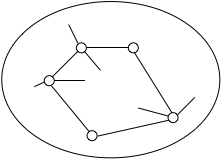
\includegraphics[scale=0.5]{FiguresGraph/EulerianProof1}
       \caption{A cycle in graph $\g$ (ignoring its other vertices and their incident edges).}
  \label{fig:eulerianProof1}
\end{center}
\end{figure}
Focus on the subgraph $\g'$ of $\g$ that is obtained by removing cycle $\cc$.  Clearly $\g'$
contains fewer than $m-2$ edges, because $\g$ has $m+1$ edges and $\cc$ contains at
least $3$ edges.

Now,  graph $\g'$ may have multiple connected components because the process of 
removing cycle $\cc$ from $\g$ could have disconnected the residual graph $\g'$; see
Fig.~\ref{fig:eulerianProof2}.
\begin{figure}[hbt]
\begin{center}
       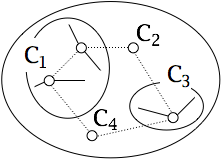
\includegraphics[scale=0.5]{FiguresGraph/EulerianProof2}
       \caption{Subgraph $\g'$ and its connected components after we removed the 
       edges of cycle $\cc$ (whose edges are dotted lines).  In this example, there are
       four connected components, $C_1$, $C_2$, $C_3$, $C_4$; two of these, namely,
       $C_2$ and $C_4$ are isolated vertices.}
  \label{fig:eulerianProof2}
\end{center}
\end{figure}
But, no matter how many components $\g'$ has, we know that each such component has no
more than $m-2$ edges.  This means that each connected component of $\g'$ is either an
isolated vertex---meaning a graph with $1$ vertex and $0$ edges---or a {\em nontrivial component},
meaning a graph that our inductive hypothesis guarantees has an Eulerian cycle.

\smallskip

The final step in extending the induction is to ``knit" the structure we have derived---namely,
cycle $\cc$ plus graph $\g'$ into  single Eulerian cycle for graph $\g$.  We accomplish this 
via the following {\em gendanken} process.  We begin to traverse cycle $\cc$, continuing
to walk until we encounter a nontrivial component, call it $\g"$, that we have never before
encountered.  We now pause in our walk along $\cc$ to traverse the Eulerian cycle in $\g"$
that the induction hypothesis guarantees.  When we conclude the traversal of $\g"$---perforce
at the same vertex where the traversal began---we resume out walk along $\cc$.  Once the
walk along $\cc$---punctuated by traversals of Eulerian cycles in connected 
components---terminates, we are guaranteed to have crossed every edges of the original graph
$\g$ exactly once.

This walk exposes the presence of an Eulerian cycle in $\g$, as claimed.   \qed
\end{proof}

\ignore{**************

The final touch is to actually \textit{construct} the eulerian cycle. 
Let start by any vertex on a cycle (thus, any vertex since they are all on a cycle...)
and to start following the cycle, as soon as we encounter a vertex in a non-empty connected component, 
we call the recursive construction on the eulerian cycle in this new component
(that is find another cycle and take the sub-connected component, and so on...).
{\Denis This is somehow what you did in your proof with the help of parameter $k$ but do we really need it?}

{\Arny Also, yesterday I inserted details for a proof similar to this in order to show that a tree has
a vertex of degree $1$ --- See Lemma~\ref{lem:vtx-deg-connected}.  Please look at that proof and 
at this proof to see whether we should craft  a single more general (abstract?) argument 
that works for both.}
{\Denis I think it is done in \ref{thm:eulerian-cycle}.
It is enough to say that the even degree vertices have at least one in-coming edge and one out-coming edge.
As the graph is connected, we simply follow a path according to the in and out edges, step by step.
This process ends up within at most $n$ steps, and may be less if it goes again through a vertex that was already considered...}

\begin{description}
\item[{\bf Step 1}]
Initialize the {\it progress parameter} $k$ to $0$.  This parameter
will help orchestrate our discovery of the Eulerian cycle within $\g$.
{\Denis no need to step 1}

\item[{\bf Step 2}]
Choose an arbitrary vertex of $\g$ some of whose incident edges have not
yet been traversed.  Call this vertex $v_k$, and let us henceforth refer
to $v_k$ as a {\em special} vertex.  Follow a walk along edges of $\g$
beginning at special vertex $v_k$.  
{\Denis we should change $v_k$ to $v$ if we change the way to write the proof...}
The rules of this walk are:
\begin{itemize}
\item
Every step of the walk will traverse an edge of $\g$ that {\em has not yet been traversed} during any walk.
\item
The walk terminates when it encounters a vertex of $\g$ {\em all of
  whose edges have already been traversed}.
\end{itemize}
The facts that 

\hspace*{.25in}\begin{tabular}{ll}
(1) & each vertex of $\g$ has even degree; \\
(2) & the walk begins at vertex $v_k$ (which crosses one of $v_k$'s edges); \\
(3) & no edge of $\g$ is traversed more than once
\end{tabular}

\noindent
mean that the last vertex encountered in this walk is $v_k$.  In other
words: {\em This walk begins and ends with vertex $v_k$.}



Note that vertex $v_k$ will occur in this walk multiple
times---specifically with multiplicity $\frac{1}{2} \mbox{\sc
  degree}(v_k)$.
  
{\Denis I would suggest here to simply a bit, in fact both  steps 1 and 2 aims simply at determining a non-empty cycle in the graph...}

We have completed the walk in $\g$ that begins and ends at vertex $v_k$.

{\Denis I suggest to skip step 3... I think it is enough -- and more easy-- to build
the whole eulerian cycle from any cycle. Do I miss something?}

\ignore{\smallskip
\item[{\bf Step 3}]
Say that we have completed the walk in $\g$ that begins at vertex $v_k$.

{\bf If} every edge of $\g$ has been traversed by the end of the
current walk, then we {\it go to {\bf Step 4}} and invoke procedure
{\bf Build Eulerian Cycle}, which stitches our series of walks into an
Eulerian cycle in $\g$.

\smallskip

{\bf Else}, there is a vertex of $\g$, call it $v_{k+1}$, one of whose
incident edges has not yet been traversed.  Note that we are here
increasing the value of our progress parameter from $k$ to $k+1$.  We
now {\it repeat {\bf Step 2}} with the updated progress parameter,
$k+1$.
}

\item[{\bf Step 4}]
\ignore{We have reached this step because our sequence of walks that begin and
end at special vertices has terminated with all of $\g$'s edges having
been traversed.}

The previous step determined a cycle in graph $\g$,.
Once it is removed, it remains several connected components,
denoted by $\mathcal{C}_1$, $\mathcal{C}_2$, $\ldots$ $\mathcal{C}_c$.
This cycle intersects the strong components at vertices $v_1$, $v_2$ until $v_c$. 
We are now ready to exhibit an Eulerian cycle in $\g$ by going piece after piece along the cycle 
starting from $v_k$.
{\Denis change it to $v$}

\end{description}

\ignore{The resulting procedure
{\bf Build Eulerian Cycle} proceeds as follows.

For each special vertex $v_k$, during the walk that begins and ends at
$v_k$, we encounter other special vertices, call them $v_{k,1}$,
$v_{k,2}$, \ldots, $v_{k,{m_k}}$, in the order of their being
encountered along the walk.  We then define the following recursive
procedure.
{\Denis it is not really recursive since each procedure is only called once...}

\medskip

\begin{tabular}{|ll|}
\multicolumn{2}{l}{{\bf Procedure Build Eulerian Cycle}($v_k$)} \\
\hline
{\bf Phase $1$} &
Follow the walk that begins at $v_k$ until it encounters $v_{k,1}$ \\
  &
Execute {\bf Build Eulerian Cycle}($v_{k,1}$) \\
\hline
{\bf Phase $2$} &
Continue the walk that begins at $v_k$ until it encounters $v_{k,2}$ \\
  &
Execute {\bf Build Eulerian Cycle}($v_{k,2}$) \\
\hline
  &
$\begin{array}{c}
\bullet \\
\bullet \\
\bullet
\end{array}
$ \\
\hline
{\bf Phase $m_k$} &
Continue the walk that begins at $v_k$ until it encounters $v_{k,m_k}$ \\
   &
Execute {\bf Build Eulerian Cycle}($v_{k,m_k}$) \\
\hline
{\bf Phase $m_k +1$} &
Complete the walk that begins at $v_k$. \\
\hline
\end{tabular}
\end{description}

\medskip

\noindent
The process invocation

Execute {\bf Build Eulerian Cycle}($v_0$)

\noindent
produces the Eulerian cycle in $\g$.
}
******************}

\medskip

We have not dealt here with the challenge of algorithmically producing the Eulerian
cycle in graph $\g$.  Our proof gives major hints about how to produce a {\em recursive}
algorithm that constructs the cycle.  Developing an iterative construction requires 
nontrivial data structuring that is outside the scope of this text.

\ignore{***********
\bigskip

When dealing with a {\em directed} graph, we proceed exactly as
with undirected graphs, with one critical difference: for each vertex
$v$ we always enter $v$ along one of its {\em in-arcs}, and
we always exit $v$ along one of its {\em out-arcs}.  As in the
undirected case, each arc is traversed precisely once during
the described process.

{\Denis my proof of the proposition is by induction on the number of edges, not vertices...}  \qed
\end{proof}
*****************}

\ignore{**************
We offer two proofs of this result: the first merely establishes the
existence of the cycle; the second actually computes the cycle.  Both
proofs invoke the following elementary facts.
\bigskip
\noindent {\bf Claim 1.}
if all the degrees are even (and not null) then there exists a cycle.\bigskip
\noindent {\bf Claim 2.}
A tour is an union of disjoint cycles.\bigskip
\noindent {\bf Claim 3.}
If we remove a cycle in a tour then the degrees remain even.\bigskip
\begin{proof}
{\bf A proof of existence.}


The necessary condition of the proposition is straightforward. 
Let us focus on the sufficient condition.
\bigskip

\noindent {\bf Proof 1 (existence).}

By contradiction, let us assume that all the vertices of a connected graph are even and there is no tour that contains all the edges.
Let consider a tour with a maximum number of edges. 
If we remove its edges, it remains some edges and from Claim~3 they are even.
Then, from Claim~1, there exists a cycle within these remaining edges (say $\Gamma$). 
The contradiction comes from Claim~2 since the union of the maximal tour plus the cycle $\Gamma$ 
is another tour which contains more edges than the initial one.
\bigskip

\noindent This proof can be adapted in a constructive way and thus, leads to an algorithm. It is as follows:

\noindent {\bf Proof 2 (constructive).}
By induction on the number of edges. 

\begin{itemize}
\item The basis case is simple to verify for $m=2$ (where two vertices linked by two edges correspond to the cycle of minimal length). 
\item
Let consider a connected graph with $m+1$ edges where all its vertices have an even degree.
Let assume that the property holds for connected graphs of even vertices with $k$ edges ($k \leq m$), which means there exist Eulerian tours in these sub-graphs. 

From Claim~1, there exists a cycle (let denote it by $\Gamma$ described by its successive vertices) and consider the sub-graph of $G$ 
without the edges of $\Gamma$: $G'=(V-{\Gamma},E')$. 
By induction hypothesis, there exists an Eulerian cycle $\mathcal{C}_i$ in each connected component of $G'$ 
(from Claim 3).
The Eulerian tour of $G$ is obtained by the concatenation of pieces of $\Gamma$ and the Eulerian cycles in the successive $\mathcal{C}_i$.

\end{itemize}
*****************}

\bigskip

The simplicity of the preceding characterization degrades a trifle when
one seeks Eulerian {\em paths} rather than {\em cycles}.

\begin{prop}[Eulerian Paths]
\label{thm:eulerian-path}
{\bf (a)}
A connected undirected graph $\g$ admits an Eulerian path if, and only if,
at most two vertices of $\g$ have odd degree.

{\bf (b)}
A connected directed graph $\g$ admits an Eulerian path if, and only if: either $\g$ admits an 
Eulerian cycle, or $\g$ contains one vertex $u$ such that

\hspace*{.5in}$\mbox{\sc indegree}(u) \ = \ \mbox{\sc outdegree}(u) +1$

\noindent
and one vertex $v$ such that

\hspace*{.5in}$\mbox{\sc indegree}(v) \ = \ \mbox{\sc outdegree}(v) -1$.
\end{prop}

The proof of the path-oriented Proposition~\ref{thm:eulerian-path} shares its overall structure
with the proof of the cycle-oriented Proposition~\ref{thm:eulerian-cycle}, with one major difference.
Whereas a cycle has neither beginning nor end, a path has both. 
Proposition~\ref{thm:eulerian-path}(a) asserts that an undirected graph which admits an
Eulerian path but not an Eulerian cycle has precisely two vertices of odd degree, and these 
odd-degree vertices play the roles of the endpoints of the Eulerian path.  In similar fashion,
Proposition~\ref{thm:eulerian-path}(b) asserts that a directed graph which admits an Eulerian
path but not an Eulerian cycle contains one vertex, $u$, whose out-degree exceeds its
in-degree and one vertex, $v$, whose in-degree exceeds its out-degree: vertex $u$ plays the role of
the beginning vertex of the Eulerian path, and vertex $v$ plays the role of the end vertex of the path.
With these hints, we invite the reader to adapt the proof of Proposition~\ref{thm:eulerian-cycle} to
obtain a proof of Proposition~\ref{thm:eulerian-path}.

\bigskip

We close this section by applying Proposition~\ref{thm:eulerian-cycle}
to the ``named graphs" of Section~\ref{sec:graphs-important-families}.

\medskip

\begin{corol}
\label{corol:eulerian-named-graphs}
The following facts about Eulerian cycles are consequences of Proposition~\ref{thm:eulerian-cycle}.

\medskip

{\small
\begin{tabular}{|l|l|l|}
\hline
Graph & Eulerian? & Explanation \\
\hline \hline
Cycle                          & Yes                          & Every vertex has degree $2$ \\
\hline
Clique                         & Odd index only       & $\k_{2n}$ has odd vertex-degrees \\
\hline
2-Dim.~Mesh  & No                           & Non-corner top and side edges have degree $3$ \\  
\hline                     
2-Dim.~Torus  & Yes                          & Every vertex has degree $4$ \\
\hline
Hypercube                  & Even index only & Every vertex of $\q_n$ has degree $n$ \\
\hline
de Bruijn                     & Yes  & Directed: Vertices have equal {\sc indegree} and {\sc outdegree} \\
                                   &         & Undirected $\d_n$: vertices $\overline{0}$ and $\overline{1}$ have
                                                  degree $2n-2$ each; \\
                                    &.       & \hspace*{.77in}all other vertices have degree $2n$ \\
\hline
\end{tabular}
}
\end{corol}

\ignore{******************
{\Denis May be we should briefly summarize what happens for these graphs 
(hypercubes with even orders, etc.)}
\medskip

The significance of the de Bruijn network in both coding and
computation (as discussed in Section~\ref{sec:deBruijn}) lends
considerable weight to the following important application of
Proposition~\ref{thm:eulerian-cycle}:  When combined with
Proposition~\ref{thm:deBruin-linegraph-EX}, we obtain a proof of 
Proposition~\ref{thm:deBruijn-Hamiltonian}.

\begin{corol}
\label{thm:deBruijn-Eulerian}
Every de Bruijn network $\d_n$ is (directed)-Eulerian.
\end{corol}
********************}

%%%%%%%%%%%%%%%%%%%%%%%%%%%%%%%%%%%%%%%%%

\subsection{Hamiltonian Paths and Cycles/Tours}
\label{sec:Hamiltonian-cycle}

We turn now to the problem of determining when a connected graph $\g$ has a
{\it Hamiltonian cycle}---and the allied problem of finding such a cycle when one exists.
Supplementary material related to cycles in general graphs, as well as in our ``named'' 
graphs can be found in the survey \cite{Rosenberg91}.

One can envision a number of benefits rendered accessible by the
presence of a Hamiltonian cycle in a graph $\g$.  Most obviously, the
cycle specifies a tour of $\g$ (or of a map whose structure $\g$
abstracts) which visits each of $\g$'s vertices precisely once.  This
is the sense in which the cycle ``summarizes" $\g$'s traversal structure.

\subsubsection{More inclusive notions of Hamiltonianicity}

Many graphs---even ones with ``nice'' structures---do not admit
Hamiltonian cycles.  The reader can generate {\it mesh-graphs}
(Section~\ref{sec:mesh}) that admit no Hamiltonian cycle.  The
existence of such non-Hamiltonian graphs has spawned several
independent paths of inquiry.  One path seeks ``modest'' ways to
weaken the property of {\it Hamiltonianicity}
\index{graph!Hamiltonianicity} in a way that retains many of
Hamiltonianicity's benefits while encompassing a broader range of
graph structures.  We describe two avenues toward weakened, more
inclusive, notions of Hamiltonianicity.

\noindent {\it Be satisfied with paths, rather than cycles}.
A {\it Hamiltonian path} \index{graph!Hamiltonian path}
\index{Hamiltonian path} in a graph $\g$ is a path that passes through
each of $\g$'s vertices precisely once.  Hamiltonian paths can easily be
shown to be a strictly weaker notion than Hamiltonian cycles, in the
obvious sense where every graph that admits a Hamiltonian
cycle also admits a Hamiltonian path: one just drops any single edge
of such a cycle to obtain such a path.  However, there are many graphs
that admit a Hamiltonian path that do not admit any Hamiltonian cycle.
As suggested earlier, there exist mesh-graphs that admit no
Hamiltonian cycle, even though every mesh-graph admits a Hamiltonian
path.  This latter claim is verified by a path that traverses the rows
of a mesh-graph {\it seriatim}, in alternating directions.

\noindent {\it Be satisfied with short paths, rather than edges}.
A Hamiltonian cycle in graph $\g$ is a circular enumeration of $\g$'s
vertices in which adjacent vertices are at unit distance from one
another---i.e., are connected by an edge.  We can weaken (or,
generalize) this notion to create a {\it Hamiltonian $k$-cycle}
\index{graph!Hamiltonian $k$-cycle} in $\g$, for any positive integer
$k$: This is a circular enumeration of $\g$'s vertices in which adjacent
vertices are at distance $\leq k$ from one another---so a Hamiltonian
$1$-cycle is what we have been calling a Hamiltonian cycle.  In fact,
the following result shows that one need not let $k$ be very big
before one encompasses all connected graphs.  Regrettably, the proof
of this result is beyond the current text.

\begin{prop}
\label{thm:weak-Hamiltonianicity}
{\bf (a)} {\rm \cite{ChartrandK69}}
Let $\g$ be any connected graph.  One can cyclically enumerate the
vertices of $\g$ in such a way that vertices that are adjacent in the cycle
are at distance $\leq 3$ in $\g$.

\index{graph!$2$-connected} \index{graph!biconnected}

\noindent {\bf (b)} {\rm  \cite{Fleischner74}}
Let $\g$ be any graph that is {\em $2$-connected} (or, {\it biconnected}) in the sense 
that, for every two vertices, $u$ and $v$, of $\g$, there exist at least two vertex-disjoint 
paths in $\g$ that connect $u$ and $v$.  One can cyclically enumerate the vertices of
$\g$ in such a way that vertices that are adjacent in the cycle are at distance $\leq 2$ in $\g$.
\end{prop}

\subsubsection{Hamiltonianicity in ``named'' graphs}
\label{sec:hamiltonian-named-graphs}

Yet another direction of inquiry is to determine whether specific
graphs of interest are Hamiltonian.  We illustrate this avenue by
reviewing the five important families of graphs we studied in
Section~\ref{sec:graphs-important-families}.

\begin{prop}
\label{thm:named-graph-Hamiltonian}
\label{thm:deBruijn-Hamiltonian}
{\bf (a)}
Every cycle-graph $\cc_n$ is Hamiltonian.

\noindent {\bf (b)}
Every clique-graph $\k_n$ is Hamiltonian.

\noindent {\bf (c)}.1.
For all $m,n$: the mesh-graph $\m_{m,n}$:

(i)  is path-Hamiltonian.

(ii) contains no odd-length cycle; hence, is not Hamiltonian if $mn$
is odd.

(iii) is Hamiltonian whenever $mn$ is even 

\noindent {\bf (c)}.2.
For all $m,n$: the torus-graph $\widetilde{\m}_{m,n}$ is Hamiltonian.

\noindent {\bf (d)}
Every hypercube $\q_n$  is Hamiltonian.

\noindent {\bf (e)}
Every de Bruijn network $\d_n$ is (directed)-Hamiltonian.
\end{prop}
 
\index{graph!pancyclic} \index{digraph!directed-pancyclic} \index{pancyclic}\index{directed-pancyclic}
Before we embark on our proof Proposition~\ref{thm:named-graph-Hamiltonian}, we
remark that some of the assertions in the Proposition can be strengthened to assert
the presence in the target graph of cycles of many lengths; cf.~\cite{Rosenberg91}.
In particular, we devote Section~\ref{Appendix:deBruijn-Pancyclic} to proving that the
$2^n$-vertex de Bruijn network $\d_n$ is {\it directed-pancyclic}---meaning that it contains
directed cycles of every length, from length $1$ to length $2^n$.

\begin{proof}[Proposition~\ref{thm:named-graph-Hamiltonian}]
\noindent {\bf (a)}
This is a tautology, by definition of $\cc_n$.

\medskip

\noindent {\bf (b)}
This is immediate because, by definition, $\k_n$ contains every
$n$-vertex graph---including $\cc_n$---as a subgraph.

\medskip

\noindent {\bf (c)}.1.i.
As we noted earlier in the text, one can ``snake'' a path through
$\m_{m,n}$, row by row, from the top-most to the bottom-most.  By
``snake'', we mean that one should traverse adjacent rows in
alternating directions.

\noindent {\bf (c)}.1.ii.
This is a consequence of the fact that $\m_{m,n}$ is {\it bipartite}:
\index{graph!bipartite} One can color $\m_{m,n}$'s vertices red and blue
in such a way that every edge connect vertices of different colors.
Details are left to the reader.

\noindent {\bf (c)}.1.iii.
We sketch the construction of a Hamiltonian cycle in $\m_{m,n}$ when
$mn$ is even.  Say, with no loss of generality that $m$ is even, so
that $\m_{m,n}$ has an even number of rows.  Temporarily remove column
$1$ of $\m_{m,n}$, and consruct the ``snaking'' Hamiltonian path
described in part {\bf (c)}.1.i of this proof.  Because $m$ is even,
this path begins and ends in column $2$ of $\m_{m,n}$.  One can,
therefore, replace column $1$ and use it to connect the ends of the
``snaking'' Hamiltonian path.  This describes a Hamiltonian cycle in
$\m_{m,n}$.

\noindent {\bf (c)}.2.
When $mn$ is even, the Hamiltonianicity of $\widetilde{\m}_{m,n}$
follows from the fact that $\m_{m,n}$ is a spanning subgraph of
$\widetilde{\m}_{m,n}$.  (Think about it!)  When $mn$ is odd, one
needs just traverse $\widetilde{\m}_{m,n}$'s vertices row by row, going
to the cyclically next vertex after completing each row (see Fig.~\ref{fig:HamiltonTorus}).  
Details of the formal proof are left to the reader.
\begin{figure}[hbt]
\begin{center}
       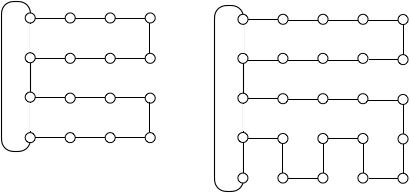
\includegraphics[scale=0.5]{FiguresGraph/HamiltonTorus}
       \caption{The principles for building Hamiltonian cycles in tori (even-even and odd-odd).}
  \label{fig:HamiltonTorus}
\end{center}
\end{figure}

\medskip

\index{Gray code} \index{binary reflected Gray code} \index{Gray, Frank}
\noindent {\bf (d)}
One can craft a Hamiltonian cycle in $\q_n$ by generating an
{\it order-$n$ binary reflected Gray code}---so named
for its inventor, Bell Laboratories researcher Frank Gray; see \cite{PetersonW81}.   
Such a ``code'' is a cyclic enumeration of all $2^n$ binary strings of length $n$, having 
the property that cyclically adjacent strings differ in only one bit-position.  Length-$n$ 
strings $x_i$ and $x_j$ are {\it cyclically adjacent} in the Gray code
$\langle x_0, \ x_1, \ldots, x_{2^n-1} \rangle$ if $j = i+1 \bmod 2^n$.
\index{strings!cyclically adjacent} 

\noindent
It is computationally easy to generate an order-$n$ Gray code from an
order-$(n-1)$ Gray code, as follows.

We note first that the order-$1$ code is the sequence $\langle 0, 1 \rangle$.

Inductively, to generate the order-$(k+1)$ Gray code from the order-$k$ code:
\begin{itemize}
\item
Concatenate the order-$k$ code with a {\em reversed} copy of itself.
(It is the code-sequence that is reversed, not the individual strings.
For instance, as we go from the order-$2$ code $\langle x_0, \ x_1,
\ x_2, \ x_3 \rangle$ to the order-$3$ code, we concatenate that
sequence with $\langle x_3, \ x_2, \ x_1, \ x_0 \rangle$.)
\item
Augment each length-$k$ string in one copy of the order-$k$ Gray code
to length $(k+1)$ by prepending a $0$ to each string; and, augment
each length-$k$ string in the other (reversed) copy of the order-$k$
Gray code to length $(k+1)$ by prepending a $1$ to each string.
\end{itemize}
The following table illustrates the first few steps of this process.
\begin{equation}
\label{eq:gray-code}
 {\small
\begin{array}{|c|c|c|c|}
\hline
\mbox{Order } \ 1
  & \mbox{Order } \ 2
  & \mbox{Order } \ 3
  & \mbox{Order } \ 4 \\
\hline
0   & 00   & 000  &  0000 \\ 
1   & 01   & 001  &  0001 \\
    & 11   & 011  &  0011 \\
    & 10   & 010  &  0010 \\
    &      & 110  &  0110 \\
    &      & 111  &  0111 \\
    &      & 101  &  0101 \\
    &      & 100  &  0100 \\
    &      &      &  1100 \\  
    &      &      &  1101 \\  
    &      &      &  1111 \\  
    &      &      &  1110 \\  
    &      &      &  1010 \\  
    &      &      &  1011 \\  
    &      &      &  1001 \\  
    &      &      &  1000 \\  
\hline
\end{array} }
\end{equation}

We now sketch a proof that for each index $n \in \N^+$, the order-$n$ Gray code sequence
specifies a Hamiltonian cycle in $\q_n$; exercises will give the reader the opportunity to fill 
in details.  We verify the following two assertions in turn:
\begin{enumerate}
\item
{\it The order-$n$ Gray code contains all $2^n$ length-$n$ binary strings.}
\item
{\it Every pair of cyclically adjacent strings in the order-$n$ Gray code differ in a single bit-position.}
\end{enumerate}
{\it Verification}.

\noindent {\it Assertion} 1.
We sketch the induction.  When $n=1$, the Gray code consists of
the two distinct strings $0$ and $1$.  Assume that the assertion holds
for $n=k$.  The order-$(k+1)$ code is obtained by taking two copies of
the order-$k$ code and prepending $0$ to the strings in one copy and
$1$ to the strings in the other copy.  The $2^k$ distinct binary
strings from the order-$k$ code thereby produce $2^{k+1}$ distinct
binary strings in the order-$(k+1)$ code.

\medskip

\noindent {\it Assertion} 2.
We distinguish three situations.  Let the adjacent strings be string $x$, which appears in 
position $i$ of the code, and string $y$, which appears in position $i+1 \bmod 2^n$ of the code.
  \begin{itemize}
  \item
Say that $i = 2^n-1$.  In this case $x$ is the last string in the
code, and $y$ is the first string.  By the ``reflective'' nature of the
construction of the code, we know that $x = 1z$ and $y = 0z$ for some
length-$(n-1)$ binary string $z$.  Strings $x$ and $y$ therefore
differ in precisely one bit-position, namely, bit-position $0$.

  \item
Precisely the same argument shows that when $i = 2^{n-1} -1$, strings
$x$ and $y$ again differ precisely in bit-position $0$.

  \item
In all other cases---i.e., when $i \in \{0,1, \ldots, 2^n-1\} \setminus \{2^{n-1} -1, 2^n-1\}$---strings 
$x$ and $y$ share the same first bit-position.  In fact, for some bit $\beta \in \{0,1\}$, 
$x = \beta u$ and $y = \beta v$ for length-$(n-1)$ binary strings $u$ and $v$ which are 
cyclically adjacent in the order-$(n-1)$ Gray code.  By an inductive argument, $u$ and $v$ 
differ in precisely one bit-position---which means that $x$ and $y$ also differ in precisely one bit-position.
  \end{itemize}
The previous analysis is summarized in Fig.~\ref{fig:HamiltonHypercude} for $n=4$.
  \begin{figure}[hbt]
\begin{center}
       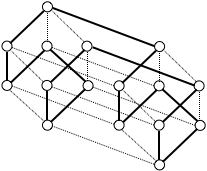
\includegraphics[scale=0.6]{FiguresGraph/HamiltonHypercube}
       \caption{A Hamiltonian cycle (bold) in $\q_4$ built using a
       binary reflected Gray code.}
  \label{fig:HamiltonHypercude}
\end{center}
\end{figure}

\noindent {\bf (e)}
de Bruijn networks require the most complex analysis of Hamiltonianicity among our  ``named" graphs .  
We begin to deal with them by restating the result in more detail in order to establish some notation.

\smallskip

\noindent
{\em
For all $n \in \N^+$, $\d_n$ contains a {\em directed Hamiltonian cycle}, i.e., a length-$2^n$ 
directed cycle of the form
\begin{equation}
\label{eq:deBruijn-cycle}
 x \ \rightarrow \ y_1 \ \rightarrow \ y_2 \ \rightarrow \cdots \ \rightarrow \ y_{2^n-1} \ \rightarrow \ x
\end{equation}
which contains every vertex of $\d_n$ precisely once; i.e.:
\begin{itemize}
\item
$\{x, \ y_1, \ y_2, \ldots, \ y_{2^n-1}\} \ = \ \n_{\fd_n}$.
\item
All of the vertices $y_j$ that appear in cycle (\ref{eq:deBruijn-cycle}) differ from $x$ and from each other.
\end{itemize}
}

The simplest proof of this result has two steps.  The first step introduces a significant, rather
sophisticated, concept, the {\it line (di)graph}.

\bigskip

\index{line graph} \index{line digraph}

\noindent {\bf (1)}
For any directed graph $\g$, the {\it line digraph} of $\g$, denoted $\Lambda(\g)$, is the
following directed graph.
\begin{itemize}
\item
The vertices of $\Lambda(\g)$ are the arcs of $\g$:
\[ \n_{{\Lambda}({\cal G})} \ = \ \a_{\fg} \]

\item
For each pair of arcs of $\g$ of the form
\[ \big[a_{x,y} = (x \ \rightarrow \ y) \big] \ \ \ \mbox{ and } \ \ \ 
\big[a_{y,z} = (y \ \rightarrow \ z) \big]
\]
i.e, arcs such that the target of the first arc is the source of the
second arc, $\Lambda(\g)$ contains an arc $(a_{x,y} \ \rightarrow \ a_{y,z})$.
\end{itemize}
The relevance of this concept to this section is that the line graph of every de Bruijn network
$\d_n$ is the ``next bigger'' de Bruijn network, $\d_{n+1}$.  Let us verify this claim.

\begin{lemma}
\label{thm:deBruin-linegraph}
For all $n \in \N^+$, $\d_{n+1}$ is the line digraph of $\d_n$; symbolically,
\[ \d_{n+1} \ = \ \Lambda(\d_n) \]
\end{lemma}

\begin{proof}[Lemma~\ref{thm:deBruin-linegraph}]
Each vertex of $\Lambda(\d_n)$ is an arc of $\d_n$, hence has the form
\[ (\beta x \ \rightarrow \ x \gamma) \]
where $x$ is a length-$(n-1)$ binary string and $\beta, \gamma \in \{0,1\}$.  Let us 
associate vertex $\beta x \gamma$ of $\d_{n+1}$ with this vertex of $\Lambda(\d_n)$.
See Fig.~\ref{fig:dBlabelEdge-App}.
\begin{figure}[hbt]
\begin{center}
       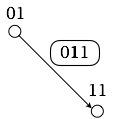
\includegraphics[scale=0.5]{FiguresGraph/dBlabelEdge}
\caption{Illustrating how to label each arc of a de Bruijn network by concatenating the labels
of the vertices incident to the arc and compacting the common intermediate bits.  In the 
depicted example, the vertex-labels $01$ and $11$ combine to yield the arc-label $011$.}
  \label{fig:dBlabelEdge-App}
\end{center}
\end{figure}

\smallskip

Note first that each arc of $\d_{n+1}$ has the form
\[ (\delta y \varepsilon \ \rightarrow \ y \varepsilon \varphi), \]
where $y$ is a length-$(n-2)$ binary string and $\delta, \varepsilon, \varphi \in \{0,1\}$.  
By our association of vertices of $\d_{n+1}$ with arcs of $\d_n$, this arc of $\d_{n+1}$ does, 
indeed, correspond to two successive arcs of $\d_n$.   The first of these successive arcs
{\em enters} vertex $y \varepsilon$ of $\d_n$; the second {\em leaves} that vertex.

Note next that, given any two successive arcs of $\d_n$, say
\[
(\rho \sigma z \ \rightarrow \ \sigma z \tau) \ \ \ \mbox { and } \ \ \
(\sigma z \tau \ \rightarrow \  z \tau \xi)
\]
where $z$ is a length-$(n-2)$ binary string and $\rho, \sigma, \tau,
\xi \in \{0,1\}$, there is, indeed, an arc of $\d_{n+1}$ of the form
\[ (\rho \sigma z \tau \ \rightarrow \ \sigma z \tau \xi) \]
This means that the digraph $\d_{n+1}$ is identical to the digraph
$\Lambda(\d_n)$, except for a renaming of vertices and arcs.\footnote{Technically,
  we are asserting that the digraphs ${\cal D}_{n+1}$ and ${\Lambda}({\cal D}_n)$ 
  are {\it isomorphic} to one another.  The topic of graph isomorphism is beyond the 
  scope of this text, but our informal description provides all the details one would 
  need to formalize the described isomorphism.}

The just-described correspondence between the vertices and arcs of digraphs $\d_{n+1}$
and $\Lambda(\d_n)$ completes the proof.  \qed-Lemma~\ref{thm:deBruin-linegraph}
\end{proof}

\medskip

\index{Eulerian cycle} \index{Eulerian tour} 

\noindent {\bf (2)}
The table following Proposition~\ref{thm:eulerian-cycle} contains the seeds of a proof of
the following corollary to the proposition.

\begin{corol}
\label{thm:deBruijn-Eulerian}
Every de Bruijn network $\d_n$ admits a (directed) Eulerian cycle.
\end{corol}

This corollary combines with Lemma~\ref{thm:deBruin-linegraph} to complete the proof of 
Proposition~\ref{thm:named-graph-Hamiltonian}(e).  To wit:  Each $\d_n$ is the line-digraph of  $\d_{n+1}$. 
Therefore, by definition of  ``line (di)graph'', the fact that $\d_n$ is (directed)-Eulerian
(Corollary~\ref{thm:deBruijn-Eulerian}) means that $\d_{n+1}$ is (directed)-Hamiltonian.  \qed
\end{proof}


\subsubsection{Testing general graphs for Hamiltonianicity}
\label{sec:Hamiltonian-unweighted}

The techniques we use in Section~\ref{sec:hamiltonian-named-graphs} to investigate 
the Hamiltonianicity of our ``named'' graphs exploit the detailed structures of the individual 
graphs.  Thus, we cannot expect the proof of Proposition~\ref{thm:named-graph-Hamiltonian} 
to suggest avenues for determining whether an arbitrary given graph is Hamiltonian.  In
fact, quite sophisticated results proved in the early 1970s make a strong mathematical
argument that no set of case studies is likely to have a major impact on the problem of 
testing general graphs for Hamiltonianicity.  This is because, in common with the Satisfibility
problem {\sf 3SAT} of Section~\ref{sec:Satisfiability}, the Hamiltonianicity-detection problem is 
{\sf NP}-complete.  We repeat from our discussion in Section~\ref{sec:Satisfiability} that the
details of the theory of {\sf NP}-completeness are beyond the scope of
this text, but we do want the reader to recognize the following.
\begin{description}
\item
{\it The problem of deciding, given a graph $\g$ that is presented via a list of vertices and a 
list of edges, whether $\g$ admits a Hamiltonian path or a Hamiltonian cycle is {\sf NP}-complete.}
\end{description}


%%%%%%%%%%%%%%%%%%%%%%%%%%%%%%%%%%%

\section{$\oplus$ Pointers to Advanced Topics}
\label{sec:advanced-topics}

%**PROVIDE SOME REFERENCES

We conclude this chapter by mentioning a variety of topics that are typically not covered---at least in depth---early in the curriculum, but that are important enough that the reader should at least be aware of them.  The topics we mention are motivated by virtually every computational area that benefits from graph-theoretic models.  We have tried to present each topic at a level of discourse that will prepare the interested reader to delve more deeply into the material, yet at a level of informality that will make the material accessible to the more casual reader.  We thus strive for an intuitive presentation that will not lead any reader astray.

%The problem that we discuss in Section~\ref{sec:Relate-CS-Math-Probs}
%illustrates how the {\em dynamic} models in the field of
%algorithmics---``dynamic'' in the sense that they {\em do}
%something---and the {\em structural} models provided by graph theory
%can often provide beneficial illumination of one another.

\index{graph!graph separators}\index{graph!graph decomposition}

Section~\ref{sec:graph-decompose} focuses on the myriad computations on graphs that can be accomplished efficiently via recursive algorithms that decompose, then reassemble, the graphs that they work on.

\index{graph!evolving graphs}
Section~\ref{sec:graph-evolve}  introduces the increasingly important topic of graphs whose structure changes dynamically over time.  One timely instance of such dynamic evolution is the connectivity graph of the Internet.

\index{hypergraphs} \index{graph!hypergraphs}

Section~\ref{sec:hypergraphs} introduces {\it hypergraphs}, a generalization of graphs that allows relationships among {\em multiple} entities, in contrast to the restriction to {\em binary} relationships imposed by graphs' {\em two-element} edges.  Hypergraph-based models find application in areas as diverse as:
\begin{itemize}
\item
{\it social networks:} Hyperedges can describe, e.g., collaboration and collusion.
\item
{\it electronic networks:} Hyperedges can enable the design of equi-potential vertices in 
voltage-driven technologies such as {\it VLSI}.
\item
{\it communication networks:} Hyperedges can model bus-oriented communication.
\end{itemize}

\index{graph!multigraphs}
\index{multigraphs}

Section~\ref{sec:multigraphs} introduces {\it multigraphs}, a generalization of graphs which allows a graph to have multiple edges connecting each pair of vertices.  In contrast to graph generalizations such as hypergraphs, multigraphs are used more {\em internally}, as an algorithmic device, than {\em externally}, as an abstraction that models features of ``real'' structures.  We introduce multigraphs here as a formalism for dealing algorithmically with edges that are weighted by integers: An edge with weight $c \in \N^+$ that connects vertices $u$ and $v$ is modeled by having $c$ unweighted edges connecting $u$ and $v$.  Of course, this is a rather primitive genre of ``modeling'', but it does afford one two equivalent ways to think about the situation---and such an option can trigger algorithmic ideas.


%\subsection{Relating Computational and Mathematical Problems}
%\label{sec:Relate-CS-Math-Probs}

\subsection{Graph Decomposition}
\label{sec:graph-decompose}
\index{graph!decomposition}
\index{graph!bisector}
\index{graph!separator}

The reader will certainly have noted that some ``named'' graphs are, intuitively, more  tightly interconnected than others.  From a purely intellectual vantage point, it would  be of interest to be able to quantify the tightness of such interconnectedness.  Among  the various measures that have been proposed, one stands out for its myriad algorithmic implications: the notion of {\it graph separator}.  In fact, this notion appears in the literature in several flavors.  An $n$-vertex, $e$-edge graph $\g$ has:
\begin{itemize}
\item
an {\it $\alpha$-edge separator} of size $k$---where $\alpha$ is a real number with $\alpha \leq 1/2$  and $k$ is an integer with $k < n$---precisely if:
\index{graph!$\alpha$-edge separator of size $k$}

\smallskip

one can partition $\g$ into two disjoint (not-necessarily connected) subgraphs, each having 
$\leq \alpha n$ vertices, by removing $\leq k$ edges from $\g$.

\item
a {\it $\alpha$-vertex separator} of size $\ell$, where $\alpha$ is a real number with  $\alpha \leq 1/2$ and $\ell$ is an integer with $k < e$, precisely if:
\index{graph!$\alpha$-vertex separator of size $\ell$}

\smallskip

one can partition $\g$ into two disjoint (not-necessarily connected) subgraphs, each having
$\leq \alpha n$ vertices, by removing $\leq \ell$ vertices from $\g$.
\end{itemize}
We replace the term ``separator'' with the term {\em ``bisector''}  if both subgraphs after a 
separation operation have $\leq \left\lfloor \frac{1}{2} n \right\rfloor$ vertices.
\index{graph!edge bisector} \index{graph!vertex bisector}

\medskip

Commonalities and differences in inherent separator sizes are often not visually obvious.  For illustration, referring to the ``named'' graphs of Section~\ref{sec:graphs-important-families}:
\begin{itemize}
\item
It is certainly obvious that cycles are easier to bisect than cliques, as measured by either edge or vertex bisectors.
\item
It is far less clear that de Bruijn networks and hypercubes are roughly equal in ease to bisect, as measured by vertex bisectors.
\end{itemize}
Similar separation behavior has very important algorithmic consequences.  For instance, the closeness in separation characteristics between de Bruijn networks and hypercubes manifests itself in a large range of algorithmic applications.  The range of such applications is hinted at by sources that study the algorithmics of laying out VLSI circuits (e.g., \cite{Leiserson85}) and sources that study the ability of a network's interconnections to host a range of communication patterns that enable efficient parallel computation and communication (e.g., \cite{AnnexsteinBR90,Leiserson85,Ullman84}).

\medskip

There is a large literature that develops the algorithmics of finding small separators for computationally significant families of graphs.  An early star in the firmament of such studies is the discovery in \cite{LiptonT79} of a $1/3$-vertex separator of size $\sqrt{8n}$ for $n$-vertex planar graphs.  The dual problem of finding lower bounds on the sizes of graph separators is a bit sparser but, of course, no less significant.  The reader can find a comprehensive exposition on the theory of graph separators in \cite{RosenbergH01}, including both the mathematics that
yields lower bounds on separator sizes and the algorithmics that yields upper bounds.


\subsection{Graphs with Evolving Structure}
\label{sec:graph-evolve}
\index{graph!with evolving structure}

A large variety of problems in the area of graph algorithms involve graphs---especially 
trees---whose structures evolve over time.  Such evolution is observed, e.g., in the study
of ``classical" algorithmic problems such as {\it Minimum Spanning Tree} and 
{\it Branch and Bound}; see, e.g., \cite{CLRS}.  What is certain to be more exciting to the
reader, though, are the ``modern'' topics where one encounters graphs with evolving 
structure, such as {\it social networks} and {\it inter-networks} (e.g., the {\it Internet of Things}).

For ``classical'' topics, as exemplified by the two we have mentioned, the mathematics covered in this chapter will provide the reader with the background necessary to deal with graph evolution.  Indeed, this evolution emerges as an inevitable concomitant of the algorithmics that is superimposed upon the traditional structures of graph theory: the challenge to the reader is to assimilate new algorithmic notions, not new mathematics.

\index{graph!with evolving structure!social networks}
\index{graph!with evolving structure!inter-networks}
In contrast, the ``modern'' topics we have mentioned do require the assimilation of new 
mathematics.  Dealing successfully with the algorithmic issues that arise with social 
networks and inter-networks requires the reader to understand the structures of the
evolving graph-oriented systems and how evolution changes these structures.
Among the interesting (and valuable) mathematical questions that one can pose is: 
If you are a new vertex ``applying" to join an evolving network, which vertex in the network 
is the best one to connect to, in order to best facilitate your interactions or influence within 
the community.  The latter topic leads, e.g., to the study of {\em power-law} networks.
\index{graph!with evolving structure!social networks!power-law networks}
\index{graph!with power-law degree growth patterns}

\bigskip

\noindent \fbox{
\begin{minipage}{0.95\textwidth}
An evolving network is said to {\it obey a power law} if there exists a real number $\gamma >0$
with the following property.  For all network vertices having sufficiently large vertex-degrees, the
fraction of vertices in the network that have degree $k$ is proportional to $k^{-\gamma}$.
\end{minipage}
}
\bigskip

Little of the abstract work on power-law networks would likely be studied in depth in any early course; indeed, the structure of these networks is not yet well understood even in advanced settings.  Indeed, attempts to understand power laws with rigor have given rise to a number of competing, rather sophisticated, abstract models---see, e.g., \cite{AielloCL00,BarabasiA99,Bollobas85,ChenCGJSW}---and numerous studies have attempted to understand the specific situations wherein the abstract models reflect reality more or less faithfully---see, e.g.,
\cite{BuT02,FaloutsosFF99,JaiswalRT04,TangmunarunkitGJSW02,ZeguraCD97}.


\subsection{Hypergraphs}
\label{sec:hypergraphs}
\index{graph!generalization to hypergraphs}
\index{hypergraph}

A large variety of modern computing-related topics benefit from the structure inherent in 
graph-theoretic models but do not comfortably conform to the {\em binary} relationships 
imposed by graphs' having {\em two} vertices per edge.  A model that retains the general 
structure of graph-theoretic models while it abandons the {\em binary} constraint in
edge-membership is the generalization of graphs called {\em hypergraphs}.  A hypergraph has
vertices that play exactly the same role as with graphs, but in place of a graph's $2$-element 
edges, a hypergraph has {\em hyperedges}, each being a set of vertices whose size is not
restricted to $2$.  A rather general treatment of hypergraphs can be found in the comprehensive
graph-theory text \cite{Berge73}; a specialized article that focuses on some of the topics of this 
chapter, such as vertex-coloring, is \cite{Lovasz73}.  Because of their inherent complexity, 
hypergraphs as graph-theoretic objects are usually relegated to advanced courses.
However, the literature contains many studies of hypergraphs that are ``fine-tuned'' for specific
computing-related application areas.  Many of these studies should be accessible without 
extensive mathematical background.  Sample  computing-related application areas that benefit
from hypergraph-oriented models include the following.
\begin{itemize}
\item
Bus-connected parallel communication has been part of digital-computer design since
its earliest days.  The informal picture of such a system is that there are communication 
channels which multiple agents can retrieve messages from and post messages to.  In
hypergraph-oriented terms: the vertices/communicating agents aggregate into 
groups/hyperedges.  Each group's agents share ``read/write'' access to a specific channel.  A
specialized genre of hypergraph that was invented to study the described scenario is the 
{\it interval hypergraph}  model developed in \cite{Rosenberg89a}.
\index{hypergraph!modeling bus-connected communication}
\index{hypergraph!interval hyergraph}

\item
Modern electronic circuits are implemented using integrated circuit technology, specifically, {\em VLSI: Very Large Scale Integrated circuitry}; see, e.g., \cite{Mead-Conway}.  These technologies are often voltage-driven, rather than current-driven.  Accordingly, much of the attention when designing circuits centers on the coordination of equi-potential points in a network, rather than on point-to-point transmission of signals.  Hypergraphs are tailor-made for such technologies.  A crucially important issue that arises because of the design strengths and weaknesses of VLSI 
technology is {\it fault tolerance}---how to cope with the inevitable faulty transistors in massive VLSI systems.  A variety of quite-accessible mathematical ideas can provide provocative ideas about this important topics; see, e.g., \cite{Rosenberg85a}.
\index{hypergraph!modeling integrated circuits}

\item
Social networks have become so prevalent in society that no one will be surprised to learn that many approaches to modeling the networks' interconnectivity have been studied.  In
Section~\ref{sec:graph-evolve}, we discussed an interconnectivity model based on evolving graphs and clustering within such graphs.  More recently, hypergraph-based models have also been proposed; see, e.g., \cite{Amatoetal17,LiuBV10}.
\index{hypergraph!modeling interconnectivity in social networks}
\end{itemize}

\subsection{Multigraphs and the Chinese Postman Problem}
\label{sec:multigraphs}
\index{graph!multigraph}
\index{multigraph}

A {\it multigraph} is a graph-like structure that allows a {\em multiset} of edges, rather than a set.  In detail, a multigraph $\h$ has a set $N_{\fh}$ of vertices and a {\em multiset} of edges, each being a $2$-element set of vertices.  Viewed differently, a pair of vertices in a multigraph can be connected by more than one edge.  Fig.~\ref{fig:EulerianFinal} depicts a $10$-vertex multigraph
with $3$ multi-edges.
 \begin{figure}[hbt]
\begin{center}
       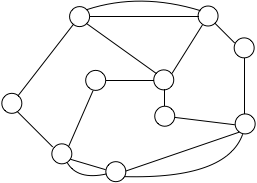
\includegraphics[scale=0.4]{FiguresGraph/EulerienFinal}
       \caption{A $10$-vertex multigraph with $3$ multi-edges.}
              \label{fig:EulerianFinal}
\end{center}
\end{figure}

\smallskip

Proposition~\ref{thm:eulerian-cycle} completely settles the ``pure'' version of the Euler-tour problem for {\em graphs}.  We learn from that result that a graph $\g$ admits a tour that crosses each edge precisely once if, and only if, every vertex $v \in N_{\fg}$ has even degree.

From an applied vantage point, pragmatism is often preferable to purity!  When one does not have access to an efficient solution for the ``pure'' version of a practically important problem, because some essential precondition is violated, then one is often willing to ``bend the rules" if such ``distortion" will give one access to an efficient solution to the resulting ``not-quite-pure'' version of the problem. 

\medskip

The preceding dictum can be illustrated via the Euler-tour problem.
\begin{description}
\item
{\em If a {\em connected} graph $\g$ has an {\em even number of odd-degree vertices}, then we can augment $\g$ by adding new edges, so that $\g$ becomes a {\em multigraph} $\g^+$ which admits a tour 
that crosses every edge precisely once.}
\end{description}
In fact, we can solve this ``distorted" version of the Euler-tour in a manner that is algorithmically efficient in the following senses.
\begin{itemize}
\item
{\em The newly added edges preserve the neighbor relation of $\g$.}

\smallskip

In other words, as we add the new edges that convert $\g$'s edge-set to an edge-{\em multiset}, we never create new adjacencies: Every new edge that we add connects vertices that were already connected in $\g$.

\item
{\em The algorithm adds the fewest number of new edges possible in order to achieve the described tour.}

\smallskip

In other words, if $\g'$ is a multigraph produced by adding edges to $\g$, and if $\g'$ has fewer edges than $\g^+$, then $\g'$ does {\em not} admit a tour that crosses each edge precisely once.
\item
{\em The algorithm is computationally efficient: it operates in time polynomial in the size of the graph $\g$.}
\end{itemize}

\medskip

\index{Route Inspection Problem} \index{Chinese Postman Problem} \index{Kwan Mei-Ko}

Our ``distorted" version of the Euler-tour problem is actually a well-known combinatorial optimization problem, which is known either as the {\it Route Inspection Problem} or the {\it Chinese Postman Problem}---the latter name in honor of the Chinese mathematician Kwan Mei-Ko who invented the problem \cite{Kwan60}.  These colorful names arise from stories about a person---either a route inspector or a postal employee---who must traverse all of the roads in a village and who wants to avoid extraneous road traversals.

\ignore{******************
A postman moved recently from Grenoble to a small village in the country side. 
He asked himself how to organize his daily tour by bike for distributing the letters in the shortest possible time. 
The director of the post office gives him the map and 
fortunately, the postman had some old souvenir of previous lectures in Graph Theory.  
The tour starts from the post office and of course, the postman has to go through every roads for distributing the letters before coming back
to his office.
The underlying graph is $G=(V,E)$ where $V$ is the (finite) set of cross points and $E$ is the set of the links between the cross roads
weighted by the distances.  
************}

\medskip

We illustrate the problem and an algorithm that solves it.

\smallskip

Fig.~\ref{fig:EulerianInitial} presents a $10$-vertex input $\g$ to our ``distorted" Euler-tour problem. 
\begin{figure}[hbt]
\begin{center}
       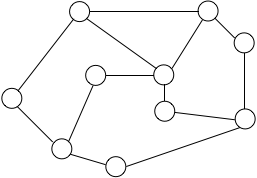
\includegraphics[scale=0.4]{FiguresGraph/EulerienInitial}
       \caption{A $10$-vertex graph which is not Eulerian.}
              \label{fig:EulerianInitial}
\end{center}
\end{figure}
Note that $\g$ is not Eulerian because it has four odd-degree vertices (happily, an even number), which are highlighted in Fig.~\ref{fig:EulerianVodd}.
\begin{figure}[hbt]
\begin{center}
       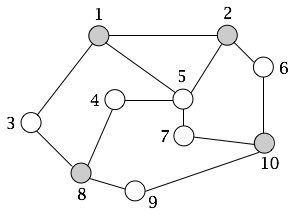
\includegraphics[scale=0.4]{FiguresGraph/EulerianVodd}
       \caption{$\g$ with its $4$ odd-degree vertices highlighted.}
              \label{fig:EulerianVodd}
\end{center}
\end{figure}

\ignore{\Arny XXX We need labeling on the vertices and edges so that we can refer to them}

\medskip

We sketch a process that adds a minimally many edges to $\g$, which converts $\g$ to a multigraph which admits a ``distorted" Euler tour. 
\begin{enumerate}
\item
Record, for each pair of vertices $u, v \in N_{\fg}$, the  length $\ell(u,v)$ of a {\em shortest path} between $u$ and $v$.  (Recall that $\g$ is connected.)

\smallskip

Computing each length $\ell(u,v)$, together with a length-$\ell(u,v)$ path between $u$ and $v$, can be accomplished efficiently, i.e., in low-degree polynomial time; see \cite{CLRS}.

\item
Say that $\g$ has $m$ odd-degree vertices $w_1, \ldots, w_m$ ($m=4$ in our illustration).  Create a copy of the $m$-clique $\k_m$ on these $m$ vertices.

\item
Label each edge $\{u,v\}$ of the clique with the path-length $\ell(u,v)$.

\item
Compute a perfect matching of minimal weight in the edge-weighted clique $\k_m$.

\smallskip

Computing minimal-weight perfect matchings can be accomplished efficiently, i.e., in low-degree polynomial time; see \cite{CLRS}.

\smallskip

Fig.~\ref{fig:Eulerianperfectmatching} illustrates the results of this process on our sample graph $\g$.   Note: the double-edges that we add make the degrees of all odd-degree vertices even.  The double-edge at the top of $\g$ in the drawing makes the degrees of both top vertices even; the length-$2$ double-edge at the bottom of $\g$ in the drawing makes the degrees of both bottom odd-degree vertices even.
\begin{figure}[hbt]
\begin{center}
       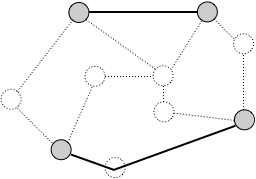
\includegraphics[scale=0.4]{FiguresGraph/EulerienPerfectMatching}
       \caption{A minimum weight perfect matching labelled by the shortest-distances $\ell(u,v)$.}
              \label{fig:Eulerianperfectmatching}
\end{center}
\end{figure}

\ignore{**********
{\Arny XXX Is something wrong here?  Why do we need a "double edge" for the two vertices at the top of the graph?  Maybe the single version of that edge should not have been in the original $\g$?  In that case, the two top vertices would have been distance-2 apart initially.}
{\Denis No all is fine since both vertices have a odd degree, thus, adding a new edge makes them even}
**********}

\item
Replace each weighted edge produced by the process by an appropriate number of multi-edges.

\smallskip

Fig.~\ref{fig:EulerianFinal} performs this last step for the weighted graph of Fig.~\ref{fig:Eulerianperfectmatching}.
\end{enumerate}

\smallskip

Our augmented multigraph $\g^+$ now has all even vertex-degrees.  We can, therefore, adapt the Euler-tour algorithm from the proof of Proposition~\ref{thm:eulerian-cycle}(a) to produce a tour of $\g^+$ that crosses each multi-edge precisely once.

\medskip

The importance of the notion of multigraph in this story is that it gave us a perspicuous bridge between the strongly algorithmic world of edge-weighted graphs and the purely graph-theoretic world that underlies Proposition~\ref{thm:eulerian-cycle}.
